\documentclass[12pt,a4paper,twoside,openright]{article}

% CREATED BY DAVID FRISK, 2015

% BASIC SETTINGS
\usepackage{textcomp}       % Fonts, symbols etc.
\usepackage{lmodern}        % Latin modern font
\usepackage{helvet}         % Enables font switching
\usepackage[T1]{fontenc}    % Output settings
\usepackage[swedish,english]{babel} % Language settings
\usepackage[utf8]{inputenc} % Input settings
\usepackage{amsmath}        % Mathematical expressions (American mathematical society)
\usepackage{amssymb}        % Mathematical symbols (American mathematical society)
\usepackage{graphicx}       % Figures
\usepackage{minted}         % Enables source code listings
\usepackage[top=3cm, bottom=3cm, inner=3cm,
  outer=3cm]{geometry}      % Page margin lengths
\usepackage{eso-pic}        % Create cover page background
\newcommand{\backgroundpic}[3]{ \put(#1,#2){
    \parbox[b][\paperheight]{\paperwidth}{
      \centering
      \includegraphics[width=\paperwidth,height=\paperheight,keepaspectratio]{#3}}}}
\usepackage{float}          % Enables object position enforcement using [H]
\usepackage{parskip}        % Enables vertical spaces correctly
\usepackage{url}
\usepackage{glossaries}


% OPTIONAL SETTINGS (DELETE OR COMMENT TO SUPRESS)

% Disable automatic indentation (equal to using \noindent)
\setlength{\parindent}{0cm}


% Caption settings (aligned left with bold name)
\usepackage[labelfont=bf, textfont=normal,
  justification=justified, singlelinecheck=false]{caption}


% Activate clickable links in table of contents
\usepackage{hyperref} \hypersetup{colorlinks, citecolor=black,
  filecolor=black, linkcolor=black, urlcolor=black}


% Define the number of section levels to be included in the t.o.c. and
% numbered (3 is default)
\setcounter{tocdepth}{5}
\setcounter{secnumdepth}{5}


% Chapter title settings
\usepackage{titlesec}
\titleformat{\chapter}[display]
  {\Huge\bfseries\filcenter}
  {{\fontsize{50pt}{1em}\vspace{-4.2ex}\selectfont
      \textnormal{\thesection}}}{1ex}{}[]


% Header and footer settings (Select TWOSIDE or ONESIDE layout below)
\usepackage{fancyhdr}
\pagestyle{fancy}


% Select one-sided (1) or two-sided (2) page numbering
\def\layout{2}	% Choose 1 for one-sided or 2 for two-sided layout
% Conditional expression based on the layout choice
\ifnum\layout=2	% Two-sided
    \fancyhf{}
	\fancyhead[LE,RO]{\nouppercase{ \leftmark}}
	\fancyfoot[LE,RO]{\thepage}
	\fancypagestyle{plain}{			% Redefine the plain page style
	\fancyhf{}
	\renewcommand{\headrulewidth}{0pt}
	\fancyfoot[LE,RO]{\thepage}}
\else			% One-sided
  	\fancyhf{}
	\fancyhead[C]{\nouppercase{ \leftmark}}
	\fancyfoot[C]{\thepage}
\fi


% Enable To-do notes
\usepackage[textsize=tiny]{todonotes}   % Include the option "disable" to hide all notes
\setlength{\marginparwidth}{2.5cm}


% Supress warning from Texmaker about headheight
\setlength{\headheight}{15pt}


\date{\today}

\begin{document}

\pagenumbering{roman}

% CREATED BY DAVID FRISK, 2015

% COVER PAGE
\begin{titlepage}
\newgeometry{top=3cm, bottom=2.7cm,
  left=2.25 cm, right=2.25cm}	% Temporarily change margins

% Cover page background
\AddToShipoutPicture*{\backgroundpic{-4}{56.7}{figure/auxiliary/frontpage_swe.pdf}}
\addtolength{\voffset}{2cm}

% Cover picture (replace with your own or delete)
% \begin{figure}[H]
% \centering
% \vspace{2cm}	% Adjust vertical spacing here
% \includegraphics[width=0.9\linewidth]{figure/Wind.png}
% \end{figure}

% Cover text
\mbox{}
\vfill
\renewcommand{\familydefault}{\sfdefault} \normalfont % Set cover page font
\textbf{{\Huge Programmering som\\ undervisningsverktyg för Transformer,\\signaler och system\\[0.2cm]}}
{\Large Utvecklingen av läromaterialet \textit{TSS med DSL} }\\[0.5cm]
Kandidatarbete inom Data- och Informationsteknik \setlength{\parskip}{1cm}

\begin{flushleft}
  \Large
  Filip Lindahl\\
  Cecilia Rosvall\\
  Peter Ngo\\
  Jacob Jonsson\\
  Joakim Olsson\\
\end{flushleft}


%{\large Filip Lindah, Cecilia Rosvall, Peter Ngo, Jacob Jonsson, Joakim Olsson}
\setlength{\parskip}{2.9cm}

\textsc{Chalmers tekniska högskola} \\
\textsc{Göteborgs universitet} \\
Institutionen för Data- och Informationsteknik \\
Göteborg, Sverige, Juni 2016

\renewcommand{\familydefault}{\rmdefault} \normalfont % Reset standard font
\end{titlepage}

% IMPRINT PAGE (BACK OF TITLE PAGE)
\newpage
\thispagestyle{plain}

The Author grants to Chalmers University of Technology and University
of Gothenburg the nonexclusive right to publish the Work
electronically and in a non-commercial purpose make it accessible on
the Internet. \\
The Author warrants that he/she is the author to the
Work, and warrants that the Work does not contain text, pictures or
other material that violates copyright law.

The Author shall, when transferring the rights of the Work to a third
party (for example a publisher or a company), acknowledge the third
party about this agreement. If the Author has signed a copyright
agreement with a third party regarding the Work, the Author warrants
hereby that he/she has obtained any necessary permission from this
third party to let Chalmers University of Technology and University of
Gothenburg store the Work electronically and make it accessible on the
Internet.

\vspace{1.5cm}

\textbf{Programmering som undervisningsverktyg för Transformer, \\ signaler och system} \\
- Utvecklingen av läromaterialet \textit{TSS med DSL}


\vspace{1cm}

Filip Lindahl   \\
Cecilia Rosvall \\
Peter Ngo       \\
Jacob Jonsson   \\
Joakim Olsson

\copyright ~ Filip Lindahl, 2016  \\
\copyright ~ Cecilia Rosvall, 2016\\
\copyright ~ Peter Ngo, 2016      \\
\copyright ~ Jacob Jonsson, 2016  \\
\copyright ~ Joakim Olsson, 2016
\vspace{0.5cm}

Supervisor: Patrik Jansson, Department of Computer Science and Engineering \\
Examiner: Niklas Broberg, Department of Computer Science and Engineering
\vspace{0.5cm}

Chalmers University of Technology\\
University of Gothenburg \\
Department of Computer Science and Engineering \\
DATX02-16-05 \\
SE-412 96 Gothenburg\\
Telephone +46 31 772 1000 \setlength{\parskip}{0.5cm}

\vfill
% Caption for cover page figure if used, possibly with reference to further information in the report
Typeset in \LaTeX \\
Gothenburg, Sweden 2016


\setacronymstyle{long-short-desc}

\setlength{\parskip}{2mm}
\setlength{\parindent}{0pt}

% TODOS från opponeringar.
% ==========================
%
% Generellt i rapporten
% ------------------------
% * Ta bort onödiga `vi`.
% * Mer akademiskt, mindre talspråk, exempelvis inte skriva gruppen 80 ggr.
%
% Utveckling av läromaterial
% -------------------------
% * Förklara mer om varför vi använder Bootstrap.
%
% Diskussion
% -------------------------
% * Tänk igenom hur produkten ändrades utifrån test-feedbacken.
%
% Referenser
% -------------------------
% * Online-resurser ska ha en `Läst den` grej.
% * Sidanvisningar till böcker för specifika saker som citat.


\section*{Förord}
Denna rapport behandlar kandidatarbetet ``Matematikens domänspecifika
språk (DSLsofMath) för andra kurser'' som genomfördes på Chalmers
tekniska högskola under vårterminen 2016. Vi som har gjort detta
kandidatarbete är fem studenter från civilingenjörsprogrammen
Datateknik och Teknisk Matematik på Chalmers.

Vi vill tacka Patrik Jansson, vår handledare, som har varit väldigt
hjälpsam och skickat oss i rätt riktning när vi varit vilsna. Vi vill
tacka Adam Sandberg Eriksson som har svarat på frågor vi haft och
funnits tillgänglig när vi undrat saker. Vi vill tacka Bo Egardt och
Ants Silberberg som tagit sig tid att diskutera sina kurser med
oss. Och slutligen vill vi tacka vår fantastiska testgrupp som gått
igenom vårt material och gett oss återkoppling för att förbättra vår
produkt.

\newpage

\thispagestyle{plain}

\section*{Sammandrag}
Denna rapport beskriver utvecklingen av läromaterialet ``\gls{tssmdsl}''
med dess tillhörande programmeringskod och lösningar. Läromaterialet
riktar sig främst till studenter inom det datatekniska programmet på
Chalmers tekniska högskola och har som syfte att vara ett
kompletterande läromedel inom signallära där man utnyttjar
studenternas kunskaper inom programmering. Materialet innehåller
förklarande text och teori om bland annat komplexa tal, signaler,
system och transformer. \\I materialet ingår även programmeringsövningar
som är skrivna med domänspecifika språk i programmeringsspråket
\gls{Haskell}. Rapporten beskriver vidare de undersökningar och efterforskningar som
gjorts för att kunna ta fram läromaterialet, samt de tester som
gjorts på den färdiga produkten.

Bakgrunden till detta projekt är att kursen inom signallära,
``Transformer, Signaler och System'', på det aktuella programmet under
många år har haft dåliga studieresultat på grund av studenternas ovana
att hantera den typ av matematik som utgör grundstommen i
kursen. Detta har visats sig inte vara något som är unikt för
data\-studenterna på Chalmers utan det är tvärtom ett problem inom många
discipliner.

Det slutliga resultatet är ett läromaterial bestående av en hemsida med
förklarande text, exempel, bilder, kryssfrågor och programmeringsövningar.
Hemsidan kan ses på \url{http://tinyurl.com/DSLsHemsida}.

Källkod och övrigt material finns på GitHub för eventuell framtida utveckling, se
\url{https://github.com/DSLsofMath/BScProj}.

\newpage

\thispagestyle{plain}

\section*{Abstract}
\selectlanguage{english}

This report describes the development of the tutorial
``\gls{tssmdsl}'' with associated programming code and solutions. The
tutorial is directed towards students studying Computer Science at
Chalmers University of Technology and the purpose of the tutorial is
to be a supplementary learning material for the course ``Transforms,
Signals and Systems''. The tutorial contains explanations and theory
concerning complex numbers, signals, systems and transforms. The
tutorial also includes programming exercises using domain specific
languages written in Haskell. The report further describes the
surveys, research and analyses done in order to produce this tutorial
and the test results from the finished product.

The background for this project is that the computer science students
studying the course ``Transforms, Signals and Systems'' have gotten
poor results for several years due to the students' unfamiliarity with
the kind of mathematics which is a large part of that course. Further
analysis has shown this to be a general problem not unique to Computer
science students at Chalmers.

The final result is a tutorial consisting of a webpage with
explanations, examples, images, quizzes and programming
exercises. The webpage can be accessed at \\
\url{http://tinyurl.com/DSLsHemsida}

The source code and other material is also available on GitHub for
possible further future development, see
\url{https://github.com/DSLsofMath/BScProj}.

\newpage

\selectlanguage{swedish}
\tableofcontents

\newpage

% Fit glossary in one page
\setlength{\parskip}{1mm}
\glossarystyle{altlist}
\printglossaries

\newpage

\setcounter{page}{1}
\pagenumbering{arabic}			% Arabic numbering starting from 1 (one)
\setlength{\parskip}{2mm plus2mm}

\section{Inledning}
Detta kapitel beskriver bakgrunden till projektet och hur det
uppstod, samt projektets mål och rapportens syfte.

\subsection{Bakgrund}
\label{sec:bakgrund}
Det finns flera studier som visar på att det matematiska språket
används på ett för otydligt sätt i undervisningssammanhang och att man
antar att studenterna är betydligt mer vana vid och bevandrade i
matematiken än de oftast är \cite{sussman2002role}
\cite{wells1995communicating}. Detta gör att vissa grundläggande
detaljer, som då antas vara allmän kunskap, utelämnas och de studenter
som inte är tillräckligt vana vid matematik får inte helhetsbilden.
Det huvudsakliga problemet är alltså inte språket i sig utan att det
ofta används på fel detaljnivå. Hur ska man då veta på vilken nivå man
bör lägga sina förklaringar? En lösning som Sussman och Wisdom
föreslår i sin studie \textit{The role of programming in the
  formulation of ideas} \cite{sussman2002role} är att försöka förklara
för en dator, om en dator förstår konceptet är förklaringen
tillräckligt detaljerad.

Ett exempel på detta problem går att finna på Chalmers tekniska
högskola. Där finns det en lång trend där studenterna på utbildningen
för Datateknik har haft svårigheter med kurserna \textit{\gls{tss}}
och \textit{\gls{regler}}. Svårigheterna med dessa kurser tror
examinatorerna till stor del beror på att studenterna inte är
tillräckligt bekväma i det matematiska språket.
% Detta syns bland annat i statistiken av hur många datastudenter som
% klarar kurserna.

Inspirerat av artiklar av bland andra Sussman, Wisdom och Wells
påbörjades ett pedagogiskt projekt på Chalmers, \textit{\gls{dslm}},
vars syfte var att minska svårigheterna som studenterna hade med
kurserna \gls{gls-tss} och \gls{regler}. Projektet har resulterat
hittills i en kurs som heter \textit{\gls{dat325}}. Kursen gavs första
gången våren 2016 och är i skrivande stund i utvärderingsfasen. I
kursen får studenterna angripa matematiska problem och försöka lösa
dem med ett verktyg de är mer familjära med än matematik, nämligen
funktionell programmering. Språket som används i kursen är
Haskell. Studenterna har tidigare varit i kontakt med Haskell och
språket har dessutom en notation med fokus på tydlighet som lämpar sig
väl för att lära ut matematiska begrepp
\cite{TFPIE15_DSLsofMath_IonescuJansson}.

Detta kandidatprojekt uppstod som en avgrening ur
\gls{gls-dslm}-projektet med fokus på att utveckla material till
specifika kurser snarare än en allmän matematisk grund.

\subsection{Rapportens syfte}
Syftet med denna rapport är att beskriva utvecklingen av
läromaterialet ``\gls{tssmdsl}'', som är ett kompletterande
läromaterial till kursen \gls{tss} för studenter på datatekniska
programmet på Chalmers, samt beskriva hur det bakomliggande problemet
kan kopplas till en mer generell problematik.

\subsection{Projektets mål}
Syftet med projektet är att underlätta för studenter inom Datateknik
att ta till sig signal- och systemteoretiska ämnen genom att utnyttja
studenternas kunskaper inom programmering och även underlätta för dem
att betrakta ämnet ur en programmerares perspektiv. Tanken bakom detta
är att man ska göra gapet mellan datateknik och signalteori mindre och
minska problemen som nämns i bakgrundsavsnittet.

Projektet är tänkt att resultera i ett läromaterial som kan fungera
som ett komplement till den kurs som ges inom signalteori på den
datatekniska grund\-utbildningen. Detta läromaterial ska innehålla
förklaringar och programmeringsövningar som är anpassade för studenter
på den datatekniska utbildningen på Chalmers tekniska högskola.

\newpage

\section{Avgränsningar}
\label{sec:avgrans}
På grund av att projektet är tidsbegränsat har projektet avgränsats
till att ta fram läromaterial till endast en kurs,
\gls{tss}. Något material till kursen \gls{regler} har inte tagits fram,
annat än indirekt i form av förkunskaper. Läromaterialet som tagits
fram är ett kompletterande
material och är inte tänkt att kunna ersätta kursen eller dess
material.

% TODO: kolla upp avstavningarna - kanske någon LaTeX-inställning är
% fel? Det borde inte bli "matem-atisk", "tex-tens", etc.
Projektets fokus har under utvecklingen av materialet inte legat på
att använda ett matematiskt korrekt språk, matematiska bevis,
avancerade matematiska begrepp eller teorier. Anledningen till detta
är att materialet i första hand är tänkt att främja förståelse och
väcka intresse för ämnet. Detta beslut baserades även på boken
\textit{Didaktik för ingenjörslärare} där författarna, under en
diskussion om aktivt lärande, hävdar att:
\begin{displayquote}
``När man lär sig något kan
man få det att fastna på olika sätt. En ytligt inlärd kunskap eller
ett beteende som inte tränats tillräckligt glöms snart bort. Det är
med andra ord viktigt att metoderna tillämpas så att djuplärande
uppnås. Textens detaljer är då inte lika intressanta som textens
budskap, förståelse, sammanhang och principer. Snarare än att lära sig
'det man måste' utantill för reproduktion, sker ett personligt
tillägnande relaterat till tidigare kunskap''
\cite[s~236]{didaktik_for_ingenjorslarare}.
\end{displayquote}
I detta projekt är det alltså viktigt att ta fram ett interaktivt
material som främjar förståelse och inte fastna i detaljer.

\newpage

\section{Teknisk bakgrund}
Detta kapitel beskriver kortfattat de områden och programvara som
behövs för att bygga upp läromaterialet.

\subsection{Git och GitHub}
\gls{Git} är ett versionshanteringsprogram som gör det möjligt för
flera personer att arbeta med samma material samtidigt utan att de
skriver över varandras arbete. Så länge inte två versioner innehåller
ändringar som står i konflikt med varandra, till exempel att flera
personer samtidigt ändrar på samma rad, slås de ihop och bildar då en
tredje version vars innehåll kommer från båda de tidigare
versionerna. Alla tidigare versioner av en fil sparas och kan
återställas och man kan också återställa enstaka förändringar utan att
behöva återställa hela filen. Skulle två versioner stå i konflikt med
varandra krävs däremot en del manuellt arbete.

För ytterligare information om Git se hemsidan
\url{https://git-scm.com}.

\gls{GitHub} är en hemsida som använder Git. GitHub gör det möjligt
för utvecklare av program med öppen källkod att utveckla kod och annat
material offentligt. Öppen källkod innebär att den kod som programmet
är uppbyggt av är offentlig och tillgänglig för alla att läsa och
kontrollera.

GitHub förenklar kommunikationen mellan användare och utvecklare genom
att tillhandahålla verktyg som låter användare kommentera på enskilda
versioner av källkoden, följa upp ärenden och problem samt dokumentera
sitt projekt. GitHub har även verktyg för att underlätta samarbete
mellan utvecklare genom att man kan klona varandras projekt och bidra
med egna ändringar som huvudutvecklaren kan godkänna. Eftersom koden
lagras offentligt på GitHub så är den lättåtkomlig för andra
utvecklare vilket underlättar vid framtida vidareutveckling av kod.

För ytterligare information om GitHub se hemsidan
\url{https://github.com}.

\subsection{Funktionell programmering}
Funktionell programmering är en programmeringsparadigm där de
huvudsakliga byggstenarna är funktioner. Som Hughes nämner i sin
välciterade \textit{Why Functional Programming Matters}
\cite{hughes1989functional}, handlar funktionell programmering mycket
om att göra det möjligt att skriva så modulär kod som möjligt.
Anledningen är att det enklaste sättet att angripa ett problem är
genom att bryta ner problemet i delproblem, lösa delproblemen, och sen
sammanfoga lösningarna till en helhetslösning. Hur mycket man kan
bryta ned ett problem beror då på hur enkelt man sedan kan sammanfoga
delproblemens lösningar igen när man är klar.

Vad som gör funktioner till grundläggande byggstenar i funktionella
programmeringsspråk är att de kan skickas som parametrar till andra
funktioner, så kallade högre ordningens funktioner. Detta gör att vi
kan bygga funktioner som exempelvis bara tar hand om datastrukturer
och skicka funktionen som löser delproblemet som en parameter.

Partiell funktionsapplikation är en annan egenskap som underlättar för
funktionella programmerare att skriva mer modulär kod. Partiell
funktionsapplikation innebär att funktioner som appliceras på färre
argument än de är definierade för skapar en ny funktion, se exemplet i
figur \ref{fig:hask_partfunapp} nedan.

\begin{figure}[H]
  \begin{minted}{haskell}
    ghci> :t (+)
    (+) :: Num a => a -> a -> a

    ghci> :t (+ 1)
    (+ 1) :: Num a => a -> a

    ghci> let plusEtt = (+1)

    ghci> plusEtt 2
    3
  \end{minted}
  \caption{Figuren visar hur Haskell hanterar partiellt applicerade
    funktioner. I bilden är \mintinline{haskell}{(+)} addition som är
    definierad på två numeriska värden och
    \mintinline{haskell}{plusEtt}, \mintinline{haskell}{(+ 1)}, är en
    funktion som givet ett annat numeriskt värde adderar 1 till det.}
  \label{fig:hask_partfunapp}
\end{figure}

Haskell är ett funktionellt programmeringsspråk med stöd för partiell
funktionsapplikation, högre ordningens funktioner, algebraiska
datatyper samt lat evaluering. Lat evaluering betyder att Haskell inte
evaluerar ett uttryck förrän det behövs och detta gör det möjligt för
Haskell att hantera oändliga datastrukturer utan att processen kräver
allt virtuellt minne och terminerar.

Algebraiska datatyper är typer som består av flera andra typer. Tack
vare Haskells \textit{\gls{patternmatching}} är det lätt att definiera rekursiva
funktioner som matchar på kontruerare i de algebraiska datatyperna
vilket visas i exemplet i figur \ref{fig:hask_alg_type}.

\begin{figure}[H]
  \begin{minted}{haskell}
    data Tree a = Leaf | Node a (Tree a) (Tree a)

    mapTree :: (a -> b) -> Tree a -> Tree b
    mapTree _ Leaf = Leaf
    mapTree f (Node a l r) = Node (f a) (mapTree f l) (mapTree f r)
  \end{minted}
  \caption{Figuren visar den algebraiska datatypen
    \mintinline{haskell}{Tree a} som beskriver en trädstruktur och den
    generella funktionen \mintinline{haskell}{mapTree} som använder
    \gls{patternmatching} för att manipulera trädstrukturen.}
  \label{fig:hask_alg_type}
\end{figure}

I Haskell är det enkelt att definiera egna datatyper vilket gör att
man exempelvis kan inkapsla redan existerande typer för att göra deras
syfte mer tydligt. Man kan också med algebraiska datatyper
implementera typer som kan fungera som ett abstrakt syntaxträd. Med
högre ordningens funktioner kan man dessutom skapa generella
funktioner som arbetar på dessa typers strukturer. Detta gör att
Haskell lämpar sig bra som värdspråk för inbäddade domänspecifika
språk.

\subsection{Domänspecifika språk}
Ett \gls{dsl} är ett programmeringsspråk som till skillnad från
generella programmeringsspråk är anpassat för en specifik domän. Att
skapa domän\-specifika språk är ingenting nytt, det finns tvärtom
många \gls{dsl} som används i vid utsträckning. Exempel på några
välkända \gls{dsl} är HTML, MATLAB och Game Maker Language.

Det som är grundtanken med ett \gls{dsl} är att det är relativt enkelt
att formulera lösningar för problem inom deras domäner, exempelvis är
det enkelt att strukturera upp text i HTML, utföra matrisoperationer i
MATLAB eller skapa datorspel med Game Maker Language. Däremot är
\gls{dsl} ineffektiva inom andra områden än de som de är
implementerade för. Det är till exempel inte effektivt att försöka
skapa datorspel i MATLAB.

När man designar domänspecifika språk kan man välja att skapa ett
fristående språk som kompileras till någon typ av maskinkod eller att
utveckla sitt domänspecifika språk i ett redan existerande generellt
programmeringsspråk, där beståndsdelarna i språket är funktionsanrop
och konstruerare i värdspråket. Ett \gls{dsl} som är implementerat på
detta sätt kallas för ``\gls{edsl}''.

% TODO: Nämna att vi valde approachen EDSL
% TODO: Lägg till att det finns blandningar av djupa och ytliga EDSL.
% Det går alltså att kombinera dessa två nivåer.
Det finns även olika nivåer av \gls{edsl}; så kallade djupa \gls{edsl}
(deep embedding) och ytliga \gls{edsl} (shallow embedding). I
introduktionen till sin artikel \textit{Combining deep and shallow
  embedding for EDSL} skriver Svenningson och Axelsson
\cite{Svenningsson2012combining} att man i ett djupt \gls{edsl}
använder sig av algebraiska datatyper och att man med dessa bygger upp
ett abstrakt syntaxträd som sedan tolkas av olika funktioner. Man
definierar alltså egna typer och funktioner som bygger upp strukturer
med dessa typer och skiljer på så sätt det domänspecifika språket från
värdspråket. I ett ytligt \gls{edsl} försöker man däremot uttrycka
sitt domänspecifika språk i termer av värdspråkets funktioner och
typer. Ett uttryck i ett ytligt \gls{edsl} motsvaras alltså av ett
uttryck i värdspråket och behöver inte tolkas ytterligare. Båda sätten
att implementera ett \gls{edsl} har sina fördelar och nackdelar då det
exempelvis i ett djupt \gls{edsl} är förhållandevis lätt att ge fler
tolkningar av det abstrakta syntaxträdet och därmed kunna bygga vidare
på det domänspecifika språket, men svårare att lägga till konstruerare
eller på andra sätt ändra i typerna som bygger upp syntaxträdet
eftersom man då måste ändra i de funktioner som tolkar dem. I ett
ytligt \gls{edsl} är det lätt att lägga till konstruerare och typer
eftersom man bara måste kunna representera dem i värdspråket och
alltså inte behöver hantera ett syntaxträd, men å andra sidan är dess
tolkning fixerad. För att lägga till nya sätt att tolka ett ytligt
\gls{edsl} måste det implementeras om på nytt.

\subsection{Transformer, signaler och system}
Inom ämnet signalbehandling beskriver kursen \gls{tss} olika typer av
signaler, hur signalerna relateras till ett system och hur man kan
modellera denna relation mellan signaler och systemet i matematiska
termer. Ett system kan till exempel vara en fjäder vars insignal är en
kraft som påverkar fjädern utifrån.

I kursen, och så även i detta projekt, begränsas signalen till enbart
en oberoende variabel som beskriver tid och de system som
betraktas är linjära och tidsinvarianta, så kallade LTI-system. För
att kunna lösa problem med denna typ av signaler och system så kan man
utveckla signalen i en Fourierserie eller använda sig av olika typer
av transformer. En av de transformer som tas upp i kursen är
Fouriertransform som gör det möjligt att byta perspektiv och betrakta
signalen i frekvensdomän istället för tidsdomän.

Fouriertransform i kontinuerlig tid är definierad enligt följande:
\[\mathcal{F}[\;f\;]~\omega = \int_{-\infty}^{\infty} f(t) e^{-j \omega t} dt\]

Området transformer, signaler och system innehåller även andra begrepp
och operatorer som komplexa tal, faltning, sampling med flera. Alla
dessa grundkunskaper behövs för att modellera system och signaler.

\subsection{Didaktik}
\label{sec:didaktik}
Didaktik är vetenskapen om undervisning. I \textit{Didaktik för
  ingenjörslärare} \cite{didaktik_for_ingenjorslarare} hävdar
författarna att didaktik kan ses som ett komplement till pedagogik. De
didaktiska frågorna handlar, enligt författarna, inte om hur studenten
lär sig utan snarare om hur läraren skapar en situation lämplig för
lärande.

Som nämndes i inledningen har detta projekt som syfte att utveckla
läromaterial som kan fungera som ett komplement till kursen \gls{tss}
och väcka intresse för ämnet. Därför är didaktik en viktig del av
projektet.

En stor del av didaktik handlar om hur man kan påverka studentens
motivation.\\I \textit{Didaktik för ingenjörslärare} sammanfattas
motivationens betydelse enligt följande: ``Varje kurs behöver
motiveras för studenterna. Med motiverade studenter blir resultatet
bättre.''.  Boken hävdar även att långt ifrån alla studenter som går
en kurs utgår från att den är läsvärd. Även i \textit{Motivational
  Design for Learning and Performance} påpekas det orimliga i att anta
att alla studenter är motiverade att lära sig ett ämne redan när de
först kommer i kontakt med det \cite{motivational_design}. Det är
alltså viktigt att ett läromedel är uppbyggt så att det motiverar
studenterna att lära sig.

Enligt boken behöver motivations\-aktiviteter stödja inlärningsmålen
för att vara effektiva. Motivationsmedel kan vara roliga och
underhållande men om de inte engagerar studenten i läromålen och
läromaterialet så hjälper de inte studenten att lära sig. Roliga
aktiviteter och dylikt kan användas som ett belöningssystem men
främjar i sig inte lärande. Många studenter kommer även motsätta sig
eller rentav avsky aktiviteter tänkta att motivera dem om
aktiviteterna inte är knytna till läromålen, detta gäller särskilt för
vuxna studenter.  Motivationsdesign har alltså utmaningen att göra
materialet tilltalande utan att det blir ren underhållning.

Ett angreppssätt inom didaktik är \textit{ARCS-modellen}, som beskrivs
i detalj i \textit{Motivational Design for Learning and Performance}
\cite{motivational_design}. \gls{gls-arcs} är en akronym för
\textit{Attention}, \textit{Relevance}, \textit{Confidence} och
\textit{Satisfaction}, vilket är grundpelarna i
\textit{ARCS-modellen}. Nedan följer en summering av modellens fyra
grundpelare.

Den första grundpelaren \textit{Attention}, uppmärksamhet på svenska,
syftar till att väcka studentens uppmärksamhet och nyfikenhet.  Detta
åstadkoms med perceptuell stimulans, frågor och variation.
Perceptuell stimulans innebär att man på något sätt ändrar i
undervisningsmiljön för att väcka studentens uppmärksamhet. Dessa
miljöförändringar kan vara av varierande typ som till exempel en
ändring i röstläge, temperatur i en undervisningssal eller ett skämt.
Denna typ av miljöförändringar väcker dock endast en tillfällig
uppmärksamhet och måste därför följas av frågor och variation för att
ge en varaktig effekt. Därför är det viktigt att i detta skede
omedelbart följa upp med frågor som väcker studentens nyfikenhet. För
att behålla studentens nyfikenhet och intresse är det även viktigt med
variation undervisningen. Oavsett hur bra struktur man har i sin
undervisning kommer studenterna att tappa intresset om man inte
varierar upplägget.

Den andra grundpelaren \textit{Relevance}, relevans på svenska, syftar
till att övertyga studenten om att inlärningen är personligt relevant.
För att en student ska vara intresserad av att lära sig måste hen
känna att instruktionen är relaterad till personliga mål eller motiv.
Detta uppnås genom målorientering och anknytning till bekant kunskap.
Studenter är mycket mer motiverade att lära sig saker om dessa kan
hjälpa dem uppnå ett mål i nutid eller framtid, som att klara ett
prov, få en befordran, eller liknande. Därför är det viktigt att
studenterna vet hur det de lär sig är relaterat till deras mål. Ämnet
kommer även att kännas mer relevant för studenten om det kan knytas
till hens tidigare kunskap eller intresse. Även om studenter kan bli
nyfikna på helt nya saker är de som regel mest intresserade av saker
som på något sätt är knutna till deras tidigare erfarenheter.
Konkreta exempel från familjära områden gör det hela mer relevant för
studenten, detta gäller i synnerhet när man lär ut abstrakt material.

Den tredje grundpelaren \textit{Confidence}, självförtroende på
svenska, syftar både till studenters tro på att de kan ämnet och deras
tro på att de kan lära sig det. Även om en student är nyfiken på ett
ämne och känner att det är relevant är det möjligt att hen ändå inte
är tillräckligt motiverade på grund av för mycket eller för lite
självförtroende. Vissa studenter kan rentav vara rädda för ämnet. På
grund av detta är det viktigt att utveckla materialet så att studenten
övertygas om att hen kan lära sig ämnet. Därför behöver man med hjälp
av relevanta uppgifter ge studenter en upplevelse av framgång så fort
som möjligt. Detta kan vara en viktigt stimulans för fortsatt
motivation, förutsatt att uppgiften kräver så pass mycket ansträngning
att det betyder något att lyckas med den, men inte kräver så mycket
att det uppgiften leder till allvarlig oro eller hot om misslyckande.

Studentens självförtroende kan byggas upp genom lärokrav, möjlighet
till fram\-gång och personlig kontroll. Det är viktigt att sätta upp
tydliga lärokrav eftersom det är en stor källa till oro och osäkerhet
för studenten att inte veta vad som förväntas. Efter att ha
skapat en förväntan av framgång är det viktigt att ge studenten
möjlighet att lyckas med krävande och meningsfulla uppgifter. Dessa
uppgifter bör se olika ut beroende på vilken nivå studenten befinner
sig på. Studenter som är nya inom ett område reagerar generellt bäst
på om att ha en relativt låg svårighetsnivå med frekvent återkoppling
som hjälper dem lyckas eller bekräftar deras framgång. När studenter
bemästrat grunderna är de redo för mer krävande uppgifter. Slutligen
är det viktigt att studenten känner att hen har personlig kontroll
över lärandesituationen. Att uppleva att man själv kan kontrollera
utgången av en situation är avgörande för självförtroendet. För att
förstärka motivationen bör instruktören förse studenten med en stabil
lärandemiljö och sedan låta studenten ha personlig kontroll över sin
inlärning. Det är viktigt att skapa en miljö där det är acceptabelt
och helt i sin ordning att göra misstag och lära sig av dem.

Om man använder de första tre grundpelarna, Attention, Relevance och
Confidence, väl, kommer studenten vara motiverad att lära sig. Det är
för att upprätthålla denna motivation som den sista grundpelaren
\textit{Satisfaction}, tillfredsställelse på svenska, används. För att
studenten ska ha ett fortsatt intresse av att lära måste hen känna
tillfredsställelse med inlärningens process eller resultat. Denna
tillfredsställelse kan uppnås genom naturliga konsekvenser och
allmänna positiva konsekvenser. Med naturliga konsekvenser menas den
kunskap som blir en direkt följd av undervisningen. Att kunna lösa en
uppgift eller dylikt som man inte kunde lösa innan ger en
tillfredsställelse i sig. Det är ett starkt belöningsverktyg att låta
studenten använda ny kunskap. Allmänna positiva konsekvenser kan vara
materiella belöningar, som till exempel en löneförhöjning, eller
symboliska belöningar som diplom eller ett bara ett erkännande av
studentens förmåga.

Hur dessa didaktiska modeller och metoder har använts i läromaterialet
\gls{tssmdsl} beskrivs i avsnitt \internref{sec:utveckling}.

\subsection{Relaterad forskning}
\label{sec:relForsk}
Detta avsnitt beskriver i korthet tre studier som är nära relaterade
till detta projekt.

En studie som studerat undervisning med det matematiska språket är
\textit{The role of programming in the formulation of ideas} av Gerald
Sussman och Jack Wisdom. Sussman och Wisdom uttrycker att det är det
svårt att lära sig fysik: de resonerar att detta troligen kan bero på
att studenter tycker att det är svårt med det matematiska språket och
att det därför blir problematiskt att lära sig både ämnet och språket
som ämnet är uttryckt i \cite{sussman2002role}. De jämför det med att
försöka läsa \textit{Les Misérables} samtidigt som man försöker lära
sig franska.

Det huvudsakliga problemet med att uttrycka idéer och koncept i det
matematiska språket är dock inte språket i sig utan snarare att man,
som med naturliga språk, antar att den man talar med eller förklarar
för är van vid det matematiska språket och därför delar samma
kunskapsbas om matematik som en själv. Detta gör, enligt Sussman och
Wisdom, att man istället för att förklara matematiken så tydligt som
man bör snarare skissar upp en lösning, vilken för den matematiskt
ovane studenten blir i det närmaste obegriplig.

I artikeln föreslås en lösning på hur man hittar den detaljnivå som
krävs för att otvetydigt förklara något matematiskt är att försöka
förklara det för en dator. En dator försöker inte tänka själv och
accepterar inte halvfärdiga instruktioner där resten lämnas till
intuitionen.

En annan studie som är intressant för projektet är
\textit{Communicating mathematics: Useful ideas from computer science}
av Charles Wells \cite{wells1995communicating}. I denna artikel
argumenterar Wells för att matematiker har mycket att vinna på att
uttrycka sig tydligare. Wells drar paralleller till datavetenskapen
där man skiljer noga på syntax och semantik samt tänker explicit på
typer och hur dessa manipuleras. Detta skiljer sig från matematiken
där man inte separerar på semantik och syntax i samma grad och där
typerna oftast är implicita och lämnas till läsaren att själv fundera
på.

%Todo: Kolla igenom nedanför stycke om den är ok.
Detta projekt bygger, som tidigare nämnts, på projektet \gls{dslm} som
i sin tur bygger på idéerna från Wells, Sussman och Wisdom.  I kursen
\textit{Matematikens domänspecifika språk} får studenterna
angripa matematiska problem i ett programmerings perspektiv
genom att bygga domänspecifika språk. För att kunna göra detta måste
studenterna fundera över vad de faktiskt ska modellera och vilka typer
de kan tänkas behöva för att uttrycka problemet
med~\cite{kursplan:dslsofmath}.

\newpage

\section{Problemanalys}
Som nämndes i \internref{sec:bakgrund} är det bakomliggande
problemet till detta projekt att datastudenterna
på Chalmers har svårt för kurserna \gls{tss} och \gls{regler}.

Statistiken från Chalmers visar tydligt att kurserna \gls{tss} och
\gls{regler} har en ovanligt hög andel studenter som blir underkända
på tentamen. Under perioden 2010 till 2016 blev i genomsnitt endast
51\% av de som skrev tentamen i \gls{tss} godkända och under samma
period blev 53\% godkända i \gls{regler} \cite{tentastatistik}.
%Pajdiagram?
Det finns även ett mörkertal i dessa siffror eftersom inte alla
studenter som läser kursen skriver tentamen, exempelvis valde 48 av
122 registrerade studenter att inte tentera \gls{regler}
\cite{kursinformation:ere102:14-15}.

Kurserna i fråga, \gls{tss} och \gls{regler}, läses under tredje året
på Datateknik och kräver bland annat förkunskaper från de kurser i
matematik studenterna läser under sitt första år. \gls{regler} kräver
även förkunskaper från \gls{tss}. Det kan därför anses vara ett
rimligt antagande att bristande kunskaper i \gls{tss} orsakar
följdproblem och utgör en del av studenternas problem med
\gls{regler}. Ett läromaterial som ger ökad förståelse av \gls{tss}
skulle därför även kunna bidra till att ge ökad förståelse av \gls{regler}.

Kursernas examinatorer tror att studenternas svårigheter med
såväl \gls{tss} som \gls{regler}
till stor del beror på att studenterna inte är tillräckligt bekväma i
det matematiska språket. Se \appendixref{bil:exam_intervju} för en
sammanfattning av hela intervjun. Examinatorerna tror att studenterna
på Datateknik inte har tillräcklig vana att tolka innebörden av de
matematiska beskrivningarna och är allmänt ovana vid matematiskt
hantverk. De tror att datastudenterna därför lägger det mesta av sin
energi på att få ihop matematiken rent praktiskt, istället för att se
vad matematiken står för.

\newpage

\section{Produktspecifikation}
För att åtgärda det problem som beskrivs i föregående avsnitt har
gruppen skapat en unik produkt som är anpassad speciellt för \gls{tss}
på programmet för Datateknik på Chalmers. Den ursprungliga
produktspecifikationen som tilldelades vid arbetets start var relativt
vag. Gruppens uppgift var att ``ta fram `\gls{dslm}-inspirerat'
kompletterande material för andra närliggande kurser''. Det önskade
implementerings\-språket var Haskell och det utvecklade materialet
skulle läggas upp på GitHub.

Gruppen beslutade snabbt att fokusera på kurserna \gls{tss} och
\gls{regler} av de anledningar som nämns i problembeskrivningen. Dock
konstaterades det en bit in i projektet att tiden som fanns endast
räckte till att utveckla material av önskvärd kvalitet till en
kurs. Gruppen valde då kursen \gls{tss}, med motiveringen att
\gls{tss} innehåller förkunskaper som är nödvändiga för \gls{regler}.

\subsection{Produktens struktur}
\label{sec:prodSpec}
För att göra läromaterialet så lättillgängligt som möjligt beslutades
det
att materialet skulle samlas på en hemsida. På detta sätt kunde man
enkelt samla text, bilder och programmeringskod och presentera dem på
ett överskådligt sätt för studenterna i målgruppen.

Det beslöts att läromaterialet skulle innehålla ett antal delavsnitt
som tillsammans täckte in innehållet i kursen \gls{tss} i stora drag.
Avsikten med indelningen var att göra materialet mer överskådligt och
även göra det möjligt för studenterna att enkelt hitta aktuellt
material för ett specifikt område.

Varje delavsnitt innehåller förklaringar och exempel i löpande
text. Texten skrevs på ett sådant sätt att den är lätt att ta till sig
för målgruppen och uppmuntrar till vidare studier av ämnet.

Delavsnitten innehåller även exempel på hur det aktuella ämnet kan
beskrivas med funktionell programmering och \gls{dsl}, samt
programmeringsövningar.

\subsection{Programmeringskod och övningar}

Programmeringskoden och övningarna ska vara skrivna på ett sådant sätt att
det endast krävs grundläggande förkunskaper i funktionell
programmering och Haskell för att förstå dem. Studenten ska inte
behöva ha läst kursen \gls{dat325} eller motsvarande för att förstå
övningarna, även om det självklart underlättar.

Koden ska vara skriven för att vara lättläst och pedagogisk snarare
än att vara effektiv, eftersom koden endast är tänkt som ett läromedel
och inte ska användas för att till exempel beräkna signalers Fouriertransform
i andra sammanhang än i undervisningssyfte.

\newpage


\section{Utveckling av läromaterialet}
\label{sec:utveckling}
I detta avsnitt beskrivs hur projektgruppen gått till väga under
utvecklingen av läromaterialet, samt vilka verktyg och metoder som
använts och hur dessa tillämpats.

Enligt boken \textit{Motivational design for learning and performance}
kan man använda sig av en modell med 10 steg vid framtagningen av nytt
material till en kurs \cite{motivational_design}. Dessa 10 steg är som
följer:

\begin{enumerate}
\item Samla kursinformation. Hur ser situationen ut nu? Vad är
  nuvarande kursbeskrivning, kursmål, etc?

\item Samla information om studenterna. Vad har studenterna för
  relevanta egenskaper i form av intressen och tidigare erfarenheter
  och förkunskaper?

\item Analys av studenterna. Vad har studenterna för motivation och
  syn på kursen?

\item Analys av existerande material. Finns det någon
  motivationstaktik i det nuvarande materialet och är den i så fall
  lämplig?

\item Lista mål och utvärderingar. Vad vill jag åstadkomma och hur
  bedömer jag om jag lyckas?

\item Lista möjliga taktiker. Vilka möjliga taktiker kan uppnå de
  satta målen?

\item Välj och designa taktik. Vilken/vilka taktiker passar bäst för
  den här publiken, ämnet etc.

\item Integrera med instruktion. Hur kan jag kombinera
  motivationskomponenterna med ämnesinformationen?

\item Välj och utveckla material. Hur hittar eller skapar jag material
  för dessa mål?

\item Utvärdera och iterera vid behov. Hur kan jag utvärdera de
  väntade och oväntade effekterna av resultatet?

\end{enumerate}

Dessa steg har legat till grund för mycket av projektgruppens metodik
vid utvecklingen av läromaterialet. Gruppen inledde i enlighet med de
10 stegen med att samla in och analysera information om kursen och
målgruppen, se avsnitt \internref{sec:efterforskning}. Därefter
arbetades  en taktik enligt ARCS-modellen fram, se avsnitt
\internref{sec:matDidaktik}. Gruppen utvecklade och testade materialet,
se avsnitt \internref{sec:test}, samt utvärderade och kompletterade
det.

Gruppen hade även två inspirationskällor i form av
\textit{BetterExplained} \cite{betterexplained} och \textit{Learn You
  a Haskell for Great Good} \cite{learnyouahaskell}. Detta är två
läromaterial som projektgruppen upplevt är både informativa och
underhållande läsning.

\subsection{Inledande efterforskning och förundersökning}
\label{sec:efterforskning}

Projektgruppen inledde med litteraturstudier och efterforskningar inom
ämnet. Projektdeltagarna läste in sig på signallära, \gls{dsl},
didaktik, funktionell programmering och annan relaterad forskning.

Under projektets tidiga fas intervjuades två personer ur
personalstyrkan på Chalmers som undervisat och varit examinatorer i
kurserna \acrlong{tss} och \gls{regler}. Se
\appendixref{bil:exam_intervju} för en sammanfattning av denna
intervju. Under intervjun redogjorde examinatorerna för hur de
upplevde studenternas problem med kurserna och vad de trodde var
orsaken.

Projektgruppen sammanställde sedan en enkät, riktad till de studenter
som läst kurs\-erna \acrlong{tss} och \gls{regler}, eller skulle läsa
kurserna inom ett år. Denna enkät arbetades fram utifrån böckerna
\textit{Enkäten i praktiken} \cite{enkaten_i_praktiken} och
\textit{Enkätboken} \cite{enkatboken}.

När enkäten var framtagen användes hemsidan \textit{webbenkater.com}
för att enkelt kunna hantera och analysera studenternas svar anonymt.
Länken till enkäten skickades ut till alla datastudenter från
årgångarna 2012-2014 och 77 svar erhölls totalt. Se
\appendixref{bil:1} för ett utdrag.

Tillslut sammanställdes den insamlade informationen om
kursen, såsom kursplan, lärandemål samt de senaste årens
tentor. Utifrån kursinformationen, samt intervjun och resultatet från
enkätundersökningen, beslutades vilka områden som läromaterialet
skulle täcka.

\subsection{Läromaterialets struktur}
\label{sec:struktur}
Läromaterialet delades upp i fyra ämnesavsnitt samt en introduktion. I
introduktionen beskrivs läromaterialet övergripande samt vilka
förkunskaper som krävs. Där förklaras även konceptet \gls{dsl}. Efter
introduktionen följer det första avsnittet, vilket kort beskriver
komplexa tal och Eulers formel samt introducerar studenten till det
\gls{dsl} som används i läromaterialet. Det andra avsnittet beskriver
olika typer av signaler och deras egenskaper, det tredje beskriver
LTI-system och det fjärde och sista beskriver Fourierserier och
Fouriertransform. De ämnen avsnitten beskriver valdes, som nämns i
föregående avsnitt, utifrån information från kursen, intervjun med
examinatorerna samt studenternas enkätsvar.

Läromaterialets första ämnesavsnitt tillägnades komplexa tal. Eftersom
förståelse av komplexa tal är en viktig förkunskap till \gls{tss}
valde gruppen att inleda med repetition av detta ämne. En annan
anledning till att inleda med komplexa tal var att detta är ett område
datastudenter känner relativt väl till vid den tidpunkt i studierna då
de läser \gls{tss}. Gruppen ville ge studenterna möjlighet att bekanta
sig med det \gls{dsl} som används och hur man kan implementera
matematik med detta innan man började beskriva nytt material. Därför
ansåg gruppen att det var lämpligt att inleda med ett ämne som
datastudenterna kände sig relativt bekväma med för att de skulle kunna
fokusera på programmeringsaspekten och förstå upplägget med \gls{dsl}.

Det andra avsnittet tillägnades signaler. Signaler är ett viktigt
begrepp i kursen \gls{tss} och kunskap om signaler är en nödvändig
grund för att förstå de följande avsnitten. Därför var det ett
självklart val för projektgruppen att låta andra avsnittet handla om
detta. I avsnittet förklaras, något förenklat, med text och figurer
vad signaler är och hur några vanliga typer av signaler, som till
exempel enhetssteg, ser ut och beter sig.

Det tredje avsnittet tillägnades LTI-system. I princip alla system som
beskrivs i \gls{tss} är LTI-system. Kunskap om LTI-system och dess
egenskaper är därför avgörande för att förstå och räkna på de system
som tas upp i \gls{tss}. Avsnittet tar även upp faltning och hur detta
fungerar i LTI-system.

Det fjärde avsnittet tillägnades Fourierserier och
Fouriertransform. Dessa är centrala begrepp i kursen och något som
många datastudenter upplever som svårt. Därför valde gruppen, då det
konstaterades att det inte fanns tid att beskriva alla transformer som
finns med i \gls{tss}, att fokusera på Fouriertransform. En anledning
till detta var att Fouriertransform är nära besläktad med såväl
Laplacetransform som Z-transform och gruppen bedömde att förståelse
för Fouriertransform sannolikt skulle bidra till förståelse för de
andra två transformerna.

\subsection{Didaktik i läromaterialet}
\label{sec:matDidaktik}
Läromaterialet ska vara uppbyggt så att studenten själv får arbeta med
det utifrån sina tidigare kunskaper. Projektgrupen ville åstadkomma ett aktivt
lärande som ger studenten långvarig förståelse och intresse för ämnet,
snarare än kunskap studenten lär sig tillfälligt
utantill. \textit{Didaktik för ingenjörslärare}
\cite[s~236]{didaktik_for_ingenjorslarare} beskriver aktivt lärande enligt
följande: ``Idéen bakom aktivt lärande är att en lärprocess bygger på
en konkret erfarenhet som följs av reflektion och observation.'' Med
bakgrund av detta har projektgruppen fokuserat på att göra
läromaterialet interaktivt. Därför har enklare kryssfrågor lagts in i
texten med avsikten att låta studenten arbeta aktivt med ämnet när hen läser
teorin. Det har även lagts in programmeringsövningar där studenten
får använda och utveckla sina kunskaper i ämnet.

Det fins många didaktiska modeller som kan användas vid utveckling
av läromedel, men den som valdes för
läromaterialet TSS med DSL var ARCS-modellen. Eftersom
läromaterialet ska fungera som ett komplement till en
redan existerande kurs bedömde gruppen att det är extra viktigt att
materialet är motiverande, eftersom studenten läser det vid sidan av
sina vanliga studier. Därför ansåg gruppen ARCS-modellen var
ett bra val, eftersom den lägger stor vikt vid just motivation.
Ytterligare en anledning till att använda ARCS-modellen
var att ARCS är en didaktisk modell som var relativt lätt att
anpassa för ett skriftligt material.
ARCS-modellen beskrivs i mer detalj i avsnitt \internref{sec:didaktik}.


ARCS-modellens första grundpelare, \textit{Attention}, har
praktiserats i läromaterialet bland annat genom att använda skämtsamma formuleringar,
sammanfattningar och exempel inom ämnet. Projektgruppen har strävat efter att
hålla en lättsam och humoristisk ton för att hålla studenternas
uppmärksamhet. Dock har lustiga utvikningar,
formuleringar och exempel som avviker från ämnet eller inte fyller sin
funktion, att främja intresse och förståelse för ämnet, undvikits. För att sedan
väcka ett mer varaktigt intresse hos studenten ställes frågor i
löpande text och övningar. Varje avsnitt inleds med en fråga av typen
``Vad är det här egentligen för något och vad används det till?''. För
att behålla studentens intresse genom hela läromaterialet har upplägget
på avsnitten varierats till viss del. Eftersom det är eftertraktansvärt att
behålla en läsvänlig och överskådlig struktur i hela läromaterialet
har materialet  främst varierats med olika typer av exempel
och uppgifter. I ett kapitel får studenterna fylla i ett jämförelsevis
stort antal kryssfrågor och i ett annat fokuseras istället
på en viss typ av programmeringsövningar där studenten får fylla i
saknad kod. Målet har alltså varit att främst göra studenternas eget arbete
omväxlande för att att de inte ska bli uttråkade och ge upp.

Den andra grundpelaren, \textit{Relevance}, har praktiserats främst
i inledningen av avsnitten och i introduktionsavsnittet.
I introduktionsavsnittet förklaras att läromaterialet finns till för att
vara ett komplement till, och hjälpa datastudenterna med,
\gls{tss}. Varje ämnesavsnitt inleds sedan med en kort beskrivning av
ämnet och vad det kan användas till. På detta sätt förklaras
först varför läromaterialet är relevant för studentens
studier och Sedan förklaras vad de olika ämnesområdena
kan användas til mer i detalj efterhand som studenten stöter
på dem i materialet.

Den tredje grundpelaren, \textit{Confidence}, har praktiserats genom
att skapa övningar och uppgifter av varierande svårighetsgrad och ett
upplägg där studenten själv kontrollerar sin inlärning. Beträffande
övningarna så inlededs läromaterialet i det första avsnittet med enklare
kryssfrågor och relativt enkla programmeringsövningar. Kryssfrågorna
kan kryssas i direkt på hemsidan, varpå de rättas automatiskt för att ge
studenten omedelbar bekräftelse. Det finns även lösningsförslag till
programmeringsövningarna som studenten kan jämföra sin egen kod med alternativt
få hjälp av om hen kör fast. Eftersom det är önskvärt att studenten själv ska
kunna kontrollera sin inlärning och arbeta i en takt som fungerar för
hen passar det bra att lägga upp läromaterialet i form av en
hemsida. På så vis har studenten tillgång till all information och
alla uppgifter men kan arbeta med materialet som hen vill.

Den fjärde och sista grundpelaren, \textit{Satisfaction}, har
praktiserats främst i slutet på avsnitten och i uppgifterna. I
kryssfrågorna får studenten omedelbar bekräftelse när hen har lärt sig
något eller kan det sedan innan. Efter att studenten har läst teorin
inom ett område följs detta upp med övningar där studenten får
praktisera sin nyvunna kunskap. Varje avsnitt i läromaterialet
avslutas till sist med en lista på vad studenten nu har lärt
sig. Studenten får alltså både ett erkännande av sin kunskap och
förmåga, samt möjlighet att praktisera denna.

\subsection{Implementationen av vårt DSL}
\label{sec:implDSL}
% Förklara hur komplexa tal och alla typer av transformer
% implementerades i DSL.
Det \gls{dsl} som används i läromaterialet \gls{tssmdsl} har
utvecklats i Haskell av projektgruppen. Det har designats för att
täcka de valda delarna av \gls{tss} som behandlas i läromaterialet.

En av dessa delar är komplexa tal, vilket är ett ämnesområde som
används flitigt när man arbetar med signaler och system. Därför
implementerades komplexa tal som första byggstenen i läromaterialets
\gls{dsl}. Därefter implementerades signaler, LTI-system och
Fouriertransform.

Utvecklingen av det \gls{dsl} som använts har skett genom att all kod
som behövts för ett avsnitt först utvecklats fristående från det
övriga lärometerialet. När koden sedan hade testats och fungerade
tillfredsställande delades den upp i kodpaket. I dessa kodpaket har
vissa funktioner tagits bort för att lämnas som övningar till läsarna
att implementera. Resterande kod i paketen kan användas av studenten
så att hen kan köra sin egen kod direkt och testa sina lösningar.

Samtliga funktionerna har givits så beskrivande namn som
möjligt. Projektgruppen har även försökt åstadkomma en så lättläst
syntax som möjligt där alla implementerade funktioner kan läsas och
förstås av någon som behärskar grundläggande Haskell. Detta var
viktigt då avsikten var att åstadkomma kod som kan förstås av hela
målgruppen och inte bara av studenter som är särskilt intresserade av
Haskell.

För att visa hur projektgruppen har tänkt vid implementationen av sitt
\gls{dsl} kommer delar av implementationen av komplexa tal nu att
beskrivas. Vi börjar med hur ett komplext tal representeras, i vårt
fall som två flyttalsvärden.
\begin{minted}{haskell}
  data Complex = Complex Double Double
    deriving Eq
\end{minted}
Ett värde för den reella delen av talet och ett för den imaginära
delen. Det komplexa talet \(z = 1 + 2j = (1,2) \) representeras i vår
\gls{dsl} som:
\begin{minted}{haskell}
  Complex 1 2
\end{minted}
De implementerade komplexa talen skulle bete sig som matematikens
komplexa tal och därför var det nödvändigt att implementera diverse
beräkningsoperatorer för dem. Addition kunde implementeras relativt
enkelt då de reella delarna adderas med varandra och de imaginära med
de imaginära enligt formeln nedan \cite{conway1978functions}.
\[(a, b) + (c, d) = (a + c, b + d)\]
Vilket i Haskell implementerades så här:
\begin{minted}{haskell}
  z + w = Complex (realPart z + realPart w) (imPart z + imPart w)
\end{minted}

I kodexemplen ovan används funktioner som plockar ut den reella
(\mintinline{haskell}{realPart}) respektive den imaginära delen
(\mintinline{haskell}{imPart}) ur ett komplext tal.

Multiplikationen var lite mer komplicerad än additionen, då den
matematiska formeln för multiplikation med komplexa tal ser ut enligt
formeln nedan \cite{conway1978functions}.
\[(a, b) \cdot (c, d) = (ac - bd, ad + bc) \]
Detta implementerades enligt följande i vårt \gls{dsl}:
\begin{minted}{haskell}
  z * w = Complex (realZ*realW - imZ*imW) (realZ*imW + realW*imZ)
    where realZ = realPart z
          realW = realPart w
          imZ = imPart z
          imW = imPart w
\end{minted}

Här skapades även hjälpdefinitioner, vilka är de funktioner man finner
efter \mintinline{haskell}{where} i koden. Detta var för att undvika
att skriva samma kod om och om igen, samtidigt som det koden mer
tydlig och lättläst för studenten.

Efter att dessa operationer var färdiga så var division nästa stora
operator att implementera. Den matematiska formeln för detta ser ut
som följer:
\[ z / w = (z \cdot w') / (w \cdot w') \]
där \(w'\) är \(w\):s
konjugat. Man förlänger alltså både täljare och nämnare med nämnarens
konjugat, vilket innebär att nämnaren blir helt reell. För att
implementera division var gruppen därför tvungen att först
implementera en funktion som tar fram konjugatet av ett komplext
tal. Detta innebär att man byter tecknet på den imaginära delen av
talet. Vår funktion för det såg ut så här:

\begin{minted}{haskell}
conjugate z = Complex (realPart z) (negate (imPart z))
\end{minted}
Vår implementation av division blev då följande:

\begin{minted}{haskell}
  z / w = Complex (realPart zw' / realPart ww')
                  (imPart zw' / realPart ww')
    where zw' = z * (conjugate w)
          ww' = w * (conjugate w)
\end{minted}

En viktig förutsättning för att kunna koppla de komplexa talen till
kursen \gls{tss} var att man först implementerade Eulers formel, som
kan användas för att skapa komplexa tal utifrån en vinkel \(\phi\)
(phi). Eulers formel ser ut så här:
\[e^{j\phi}=\cos \phi+ j \cdot \sin \phi \]
Implementationen av den här representationen skedde i flera steg.
Funktionen \mintinline{haskell}{euler} skapar ett komplext tal utifrån
en given vinkel, representerad av ett flyttal.
\begin{minted}{haskell}
euler phi = Complex (cos phi) (sin phi)
\end{minted}
Enligt potenslagarna så är \(e^{a+jb} = e^{a} \cdot e^{jb}\) och
enligt Eulers formel så är \(e^{j b} = \cos b + j\cdot \sin b\).
Exponentialfunktionen för ett komplext tal kan därför implementeras
enligt nedanstående kod:
\begin{minted}{haskell}
exp z = scale (exp (realPart z)) (euler (imPart z))
\end{minted}
Sedan implementerades även trigonometriska funktioner med hjälp av
Eulers formel. \(\sin(x)\) representeras enligt följande som ett komplext
tal:
\[ \sin(x) = (e^{j x} - e^{-j x}) / 2 j \]
Vilket ser ut så här i vårt \gls{dsl}:
\begin{minted}{haskell}
sin z = (exp (j*z) - exp (-(j*z))) / (scale 2 j)
 where j = Complex 0 1
\end{minted}

Den fullständiga koden kan läsas på gruppens hemsida:

\url{https://github.com/DSLsofMath/BScProj/tree/master/Tutorial/}

Ett av de största problemen vid implementationen av signaler, och all
kod som bygger på signaler, var hur kontinuerlig tid skulle
hanteras. Kursen \gls{tss} behandlar både diskreta och kontinuerliga
signaler och det var därför önskvärt att implementera båda dessa. En
dator kan dock under normala förhållanden inte hantera kontinuerliga
funktioner utan endast diskreta.
%Osäker på hur man borde uttrycka detta för att det ska vara korrekt

Ett sätt att hantera detta är att simulera ingående data till en
kontinuerlig funktion med diskret data, där man låter avstånden mellan
de diskreta värden datan kan anta vara väldigt små. Ju mindre dessa
steg är desto bättre approximation av en kontinuerlig funktion
erhålles. Frågan som uppstår är hur lämplig en diskret approximation
är för att främja förståelsen av signaler mm i kontinuerlig tid. Se
avsnitt \internref{sec:diskussion} för vidare diskussion kring detta.

Ett annat sätt att implementera kontinuerliga fall är med djup
inbäddning och sen använda \gls{patternmatching} för att implementera
en funktion för olika signaler eller annan indata. Funktioner som
implementeras på detta sett ger svar som är mer matematiskt korrekta
än en diskret approximation. Detta ger dock inte samma möjlighet att
se mönster och att sammanfatta området i en funktion som med en
diskret approximation.

Projektgruppen valde till slut en kompromiss av dessa två angreppssätt
och använde både diskreta approximationer och \gls{patternmatching}
för att beskriva kontinuerliga fall. Gruppen har växlat mellan
varianterna beroende på vilken av dem som föreföll ge den tydligaste
förklaringen av det aktuella ämnet. Exempelvis har approximation med
diskret data använts i kapitlen om signaler och system och i kapitlet
om fouriertransform har djup inbäddning och \gls{patternmatching} använts.

\subsection{Presentation av läromaterialet}
Efter att utkast till läromaterialet utvecklats gjordes detta om till
LaTeX-format. Det var ett förhållandevis enkelt sätt att få en överskådlig
struktur och ett bra utseende på vårt läromaterial.

När de olika delarna i läromaterialet blivit färdiga så skrevs de om
till HTML, med hjälp av Pandoc, för att kunna skapa en hemsida så att
det blir mer lätt\-åtkomligt. Pandoc är ett program som översätter
text mellan olika språk. Endast ett fåtal manuella kompleteringar
krävs.  En annan fördel med att arbeta med HTML-sidor i stället för
PDF är att man kan använda sig av JavaScript, vilket ger möjligheten
att kunna göra uppgifterna interaktiva.
%Todo: Hur hanterar ni ändringar i hemsidan? ^
%Genererar ni HTML igen eller redigerar direkt?
%Erfarenhet/lärdom av detta?

Vi använde oss av jQuery, vilket är ett JavaScript-bibliotek, för att
göra det lättare att arbeta med JavaScript. jQuery är relativt lätt
att läsa och det blir därmed enklare att felsöka problem i kodningen.

Dessutom så använde vi oss av Bootstrap som stöd för hemsidan för att inte
behöva lägga alltför mycket tid på utseendet då Bootstrap har CSS kod,
som skapar själva designen av sidan. Med hjälp av denna kod så
behövdes det inte läggas lika mycket tid på designen av hemsidan utan det
löstes för det mesta direkt. Bootstrap gör det även simpelt att göra hemsidan
responsiv, vilket gör att hemsidan skalas om efter skärmstorleken utan att
spendera mycket tid för att få en läsbar design. På grund av den responsiva
hemsidan blir det möjligt att använda vilken skärm man har tillgänglig, vare
sig det är en dator eller mobil, utan att hemsidan blir dåligt optimerad,
vilket skulle distrahera läsaren bort från texten vilket aldrig är något att
sträva efter.

De figurer som gjorts till läromaterialet i form av funktionskurvor
och liknande är skapade i Matlab och \url{fooplot.com/}.

Läromaterialets delar har efter hand lagts upp på GitHub.

\subsection{Test av läromaterialet}
\label{sec:test}

För att få så givande testsvar som möjligt var det givetvis önskvärt
att testa läromaterialet på den aktuella målgruppen. Det var dock inte
möjligt att testa materialet på studenter som läste kursen samtidigt
eftersom kursen endast ges under höstterminen. Därför kontaktades
studenter som läst kursen tidigare och studenter som skulle läsa den
nästa hösttermin och hade läst de kurser som är nödvändig förkunskap.
Dessa studenter kontaktades i samband med enkäten som beskrivs i
avsnitt \internref{sec:efterforskning}. De som sedan var villiga att
delta i testandet av vår produkt lämnade en e-postadress. Detta
resulterade i en testgrupp på 13 personer.

När projektgruppen ansåg att läromaterialets tre första avsnitt var
redo att testas skickades dessa ut till testgruppen. Testningen
fungerade så att testpersonen fick ta del av materialet, arbeta med
detta och sedan ge återkoppling till projektgruppen.  Det material som
testgruppen fick innefattade texter, exempel, programkod och uppgifter
samt lösningar till uppgifterna.

När studenterna hade testat produkten och återkopplat med vad de
tyckte var bra och vad de tyckte var dåligt så bearbetades och
analyserades deras återkoppling. Utifrån testgruppens kommentarer
implementerades förbättringar för att få läromaterialet mer lättläst
och bättre anpassat till målgruppen.

Det sista avsnittet skickades inte ut till testgruppen utan
utvärderades endast internt av gruppens medlemmar då detta avsnitt
inte var klart i tillräckligt god tid för att ge testgruppen en rimlig
chans att arbeta med materialet. Den mer generella återkoppling som gavs
på de tre första avsnitten tillämpades dock även på det sista
avsnittet.

\newpage

\section{Resultat}
Projektgruppens uppgift var, vilket beskrivs i detalj i avsnitt
\internref{sec:prodSpec}, att ta fram ett kompletterande läromaterial
till \gls{tss} inspirerat av \textit{\gls{dslm}}. I detta avsnitt
beskrivs det resulterande läromaterialet och resultat från testerna.

\subsection{Läromaterialet}

%Todo: Det fjärde kapitlet kommer visas i hemsidan va?
%Det är tanken
Läromaterialet består av fyra avsnitt samt en introduktion. Avsnitten
innehåller förklarande text, bilder, kodexempel och uppgifter. Varje
avsnitt har även ett tillhörande kodpaket med förimplementerad kod
till övningarna och lösningar till dessa. De fyra avsnitten behandlar
i huvudsak komplexa tal, signaler, LTI-system och Fouriertransform.
Ytterligare avsnitt, som beskriver Laplacetransform och Z-transform,
var planerade men detta fick bortprioriteras på grund av tidsbrist.

Läromaterialet finns samlat på en hemsida, där det även är möjligt att
ladda ner materialet i form av en PDF-fil. Följ länken nedan för att
se hela materialet:
\url{https://cdn.rawgit.com/DSLsofMath/BScProj/master/Hemsida/index.html}

Bilaga \nameref{bil:3} innehåller ett delavsnitt ur läromaterialet som
beskriver \textit{Udda och Jämna signaler}. Det inleds med
övergripande definitioner och förklaringar av vad som menas med udda
och jämna signaler inom signallära, detta illustreras sedan med
figurer. Därefter följer kryssfrågor där studenten ska avgöra om den
givna signalen är jämn, udda eller ingetdera. Detta följs av ett
kodexempel där studenten får se hur man kan implementera en funktion
som avgör om en signal är udda. Studenten får sedan implementera
motsvarande funktion för jämna funktioner själv som en övning. Till
sist ges studenten två signaler att testa sina
programmeringsfunktioner på, både för detta och föregående delavsnitt.


\subsection{Testresultat}
\label{sec:testResultat}
Introduktionen och de tre första avsnitten i läromaterialet har
granskats av den testgrupp som beskrivs i avsnitt
\internref{sec:test}. Det sista avsnittet har inte granskats av
testgruppen, utan endast av projektgruppen själva samt projektgruppens
handledare. Orsaken till detta beskrivs även det i avsnitt
\internref{sec:test}.

Responsen från projektets testgrupp var genomgående
positiv. Testgruppen hävdade att de trodde att läromaterialet var ett
bra komplement till kursen.

Samtliga testsvar som kommenterade texten angav att studenterna
tilltalades av textens nivå och formuleringar. Här följer några citat
från studenter som testat materialet:
\begin{displayquote}
  ``Det lättsamma sättet som texten var skriven på gjorde att man
  inte tappade intresset.''
\end{displayquote}

\begin{displayquote}
  ``Texten var i allmänhet bra och kul att läsa, gillade den
  lättsamma tonen.''
\end{displayquote}

\begin{displayquote}
  ``Nivån är väldigt bra och att ni ibland använder monolog, där
  ni ställer en fråga och sen svarar som `en vän', gör att det känns
  mer begripligt och man får en känsla av att man pratar och
  diskuterar med en kompis om diverse ämnen. Detta ökar då förståelse
  enormt då det är annorlunda skrivet än hur till exempel föreläsare
  skriver sitt material.''
\end{displayquote}

Testgruppen ansåg även att programmeringsövningarna var begripliga och
låg på en bra nivå. Några citat från testgruppen angående övningarna
följer här:

\begin{displayquote}
  ``Övningarna känns begripliga och att ni visar vilket `out-come'
  som efterfrågas hjälper en att förstå vad exakt som behöver göras.''
\end{displayquote}

\begin{displayquote}
  ``De övningarna jag gjorde kändes lagom svåra.''
\end{displayquote}

Responsen från testgruppen innefattade även konkret kritik, exempelvis
önskade flera studenter ett annat typsnitt för övningarna än för den
övriga texten. Materialet har uppdaterats utifrån dessa önskemål och
kommentarer.

\newpage

\section{Diskussion}
\label{sec:diskussion}

Som nämns i inledningen har datateknologer svårt för kursen
\gls{tss} och enligt examinatorerna beror detta på att de har svårt för
matematiken, se \appendixref{bil:exam_intervju}. Frågor man då
kan ställa sig är vad som är orsaken till detta problem, huruvida
problemet går att lösa helt, och om det verkligen är en bra metod att
använda programmering för att lösa det?

Något som möjligen är en del av orsaken till problemet är när kursen
\gls{tss} ges. Det nuvarande upplägget på datateknologernas studier
är sådant att de läser ett antal kurser i matematik under sitt första
år, knappt någon matematik under sitt andra år och sedan läser de
\gls{tss} i årskurs tre. Det är alltså nästan ett år mellan
matematikkurserna och \gls{tss}. Denna del av problemet kan i så
fall lösas genom att till exempel ge \gls{tss} i årskurs två. Det är dock
osäkert om detta är en tillräckligt stor del av problemet för att en
förändring i kursupplägget skulle ge synbar effekt.

Under intervjun med examinatorerna
framgick det att de tror att en stor del av problemet ligger i
svårigheten att koppla den formella matematiken till dess praktiska
tolkning.

Detta skulle i så fall kunna orsaka problem när datateknologer kommer
i kontakt med matematiska läromaterial. Många matematiska texter är
uppbyggda så att de har ett inledande fokus på formell matematik, med
tyngd på matematisk korrekthet, och praktiska exempel och förklaringar
följer först senare, om alls. Ett exempel på hur en matematisk
lärotext kan vara upplagd är att man inleder med en formell
definition, följd av ett matematiskt bevis, och till sist
exempel. Denna typ av upplägg kan mycket väl fungera bra för studenter
som är vana vid formell matematik men risken är att studenter som inte
är det, till exempel datateknologer, tappar bort sig redan vid
definitionen.

I de följande delavsnitt kommer projektets metod, resultat och möjlig
framtida utveckling att diskuteras.

\subsection{Metoddiskussion}
\label{sec:metDisk}
För att utveckla ett väl fungerande läromaterial krävs goda kunskaper
inom såväl det aktuella ämnet som didaktik. Projektgruppen består dock
av fem studenter, vars erfarenhet inom området signal och systemlära
var att fyra av dem läst kursen \gls{tss}. Studenternas tidigare
kunskap i didaktik var också ytterst begränsad. På grund av detta lade
projekt\-gruppen en stor del av sin tid på nödvändig förberedande
efterforskning. Detta lämnade mindre tid till utvecklingen av
läromaterialet, vilket förorsakde att att projektgruppen inte hade
tillräckligt med tid att utarbeta ett lika utförligt material som den från
början avsett. På grund av detta inkluderades inte Z-transform,
Laplacetransform eller kursen \gls{regler} i materialet, vilket var den
ursprungliga avsikten.
%Todo: Vi nämner igen om varför vi inte tar om Z-transform och Laplacetransform
%i resultatdiskussionen. Är det ok eller känns det lite för repetitivt?

Man kan ställa sig frågan om det överhuvudtaget är en bra idé att låta
studenter ta fram den här typen av läromaterial. En nackdel är att
studenterna som skriver materialet behöver lägga en stor del av tiden
på att lära sig ämnet och nödvändig didaktik tillräckligt bra, precis
som projektgruppen har behövt göra.  En följd av detta blir dock att
studenterna får en djupare förståelse för ämnet samt får nya eller
förbättrade kunskaper inom didaktik.  Man kan rentav argumentera för
att det är ett bra läromedel just att utveckla denna typ av läromedel.

En annan fördel med ett läromaterial som utvecklas av studenter är att
dessa känner till målgruppen väl, eftersom de ingår
i den. Studenterna har därför rimligtvis lättare att sätta sig in i
vad som är svårt att förstå för en student än vad en expert inom ämnet
har. Det är också möjligt att studenter har lättare för uttrycka sig
på ett sätt som andra studenter kan förstå och ta till sig. Däremot
kommer man inte ifrån att experterna har betydligt djupare kunskaper
inom sitt ämne än studenterna och det är ytterst tveksamt att en grupp
studenter skulle kunna ta fram ett läromaterial som är på samma nivå
med lika goda insikter i ämnet som en expert. Det kan dock vara så att
den här typen av studentutvecklade läromaterial är ett bra komplement
till ämnesexperterna. En av kommentarerna från testgruppen, se avsnitt
\internref{sec:testResultat} för hela sammanhanget, påpekade just att:

\begin{displayquote}
  ``Att ni ibland använder monolog, där ni ställer en fråga och sen
  svarar som `en vän', gör att det känns mer begripligt och man får en
  känsla av att man pratar och diskuterar med en kompis om diverse
  ämnen. Detta ökar då förståelse enormt då det är annorlunda skrivet än
  hur t.ex. föreläsare skriver sitt material.''
\end{displayquote}

Denna och andra kommentarer från testgruppen är starka argument för
att denna typ av läromaterial kan fungera bra som komplement till
annan undervisning.

En stor del av utmaningen med detta projekt har varit att det inte
fanns någon uppenbar lösning på vad som skulle implementeras i
programmeringskoden. För varje område som läromaterialet tar upp har
projektgruppen behövt utvärdera vad som skulle ingå och vad som var
möjligt att implementera på en nivå som studenterna i målgruppen kan
förstå. Det har varit en ständig avvägning av att få med de mest
vitala delarna i \gls{tss} och att implementera kod som är
begriplig. \textit{The Fastest Fourier Transform in the West}
\cite{fastestfourier} är ett exempel på hur Fouriertransform kan
implementeras relativt effektivt i Haskell, men problemet är att koden
då hamnar på en nivå som överstiger förmågan hos många studenter i
målgruppen. Kod av detta slag är alltså, oavsett hur effektiv den är,
inte önskvärd i vårt läromaterial eftersom vi vill använda koden för
att förklara ett annat ämne. Om koden är för svårläst riskerar vi att
hamna i en situation där studenten varken förstår programmeringen
eller ämnet den beskriver.

När man beslutat \textbf{vad} som ska implementeras uppstår frågan
\textbf{hur} det ska implementeras. Som nämndes i avsnitt
\internref{sec:implDSL} finns det flera sätt att hantera detta. När
man arbetar med signaler finns det två grundtyper; diskreta signaler
och kontinuerliga signaler. Diskreta signaler kan implementeras
relativt enkelt, medan kontinuerliga signaler blir betydligt mer
komplicerat. Projektgruppen har under projektets gång granskat två
olika metoder för att hanterar kontinuerlig tid i
programmeringskoden. En variant är att approximera en kontinuerlig
signal med en diskret. Använder man väldigt små steg kan man få en
relativt bra approximation på detta sätt, men det är fortfarande
endast en approximation och därför blir resultatet inte fullständigt
korrekt.
En annan variant är att använda \gls{patternmatching}, där funktioner
definieras exakt för ett antal givna insignaler som definieras var för
sig. Detta ger mer korrekta svar, men ger inte samma möjlighet att
sammanfatta
området som en diskret approximation eftersom man definierar olika
fall var för sig. Detta gör det å andra sidan möjligt att definiera
typfall som studenten kan känna igen i kursen \gls{tss}.

Vad är då bäst i vårt fall, att använda en approximation som ger
större möjlighet att
sammanfatta kärnan i ämnet eller en mer matematiskt korrekt variant
som använder formler som studenten kan känna igen? Detta är en fråga
som projektgruppen inte har kunnat ta fram ett generellt svar
på. Projektgruppen har, efter mycket diskussion, valt att använda båda
varianter i läromaterialet. Vi ansåg att det fanns stora för- och
nackdelar med båda lösningarna och att de argument som vägde tyngst
berodde på vilket ämne som togs upp i det aktuella avsnittet. Inom
vissa områden avgjorde gruppen att det gav större förståelse att
sammanfatta och abstrahera, medan matematisk exakthet och typfall
bedömdes vara viktigare inom andra områden.

Som beskrivs i avsnitt \internref{sec:didaktik} är en av utmaningarna
när man utvecklar läromaterial att göra materialet tilltalande utan
att det blir ren underhållning. Detta innebär en ständig balansgång
när man utvecklar materialet. Å ena sidan vill man att materialet ska
vara så informativt och effektivt som möjligt. Å andra sidan vill man
fånga och behålla studentens intresse och uppmuntra till vidare
inlärning. Vi har i vårt material strävat efter att beakta båda
sidorna och försökt hålla en lättsam och lätt humoristisk ton utan att
överskugga det faktiska innehållet. Mer om hur detta gått diskuteras i
nästa avsnitt.

\subsection{Resultatdiskussion}
\label{sec:resDisk}
Den slutgiltiga produkten uppfyller alla delar av
produktspecifikationen med ett undantag. Ambitionen var att
läromaterialet skulle täcka in hela kursen \gls{tss}. I nuläget saknas
dock avsnitt som beskriver Laplacetransform och Z-transform. Som nämns
i avsnitt \internref{sec:struktur} prioriterades detta bort på grund
av tidsbrist i slutet av projektet. Projektgruppen hamnade i läget att
de kunde fokusera på antingen Fouriertransform eller Laplacetransform
och Z-transform. Anledningen till att gruppen valde att fokusera på
Fouriertransform var att den är nära besläktad med Laplacetransform
och Z-transform. Ur programmeringssynpunkt var det även svårt att
implementera Laplacetransform och Z-transform utan att först
implementera Fouriertransform. Det finns emellertid ett utkast till
avsnitt om Laplacetransform och Z-transform som kan utvecklas i
framtiden.

Som beskrivs i avsnitt \internref{sec:test} ställde sig testgrupppen
väldigt positiv till läromaterialet. Det är dock värt att påpeka att
testgruppen bestod av en relativt liten grupp, totalt 13 personer.
Även om testgruppens svar är en positiv indikation är det därför svårt
att dra några definitiva slutsatser om huruvida vårt läromaterial
uppnår sitt mål i nuläget.

Vidare är det så att flera personer i testgruppen går i samma årskurs
och på samma program som flera av medlemmarna i
projektgruppen. Återkopplingen kunde av praktiska skäl heller inte
vara helt anonym. Det är därför inte orimligt att anta att vissa
medlemmar i testgruppen kan ha varit partiska i sin bedömning och att
detta kan ha påverkat resultatet.

För en bättre utvärdering av läromaterialet krävs att fler studenter
inom målgruppen använder sig av det i samband med kursen
\gls{tss}. Det kommer därför dröja innan man kan se det verkliga
resultatet. Detta kan dock vara svårt att utvärdera även då eftersom
det finns många andra faktorer som kan påverka. Om en ökning i antalet
godkända studenter i kursen observeras i framtiden är det svårt att
säga med säkerhet i vilken utsträckning denna förändring beror på vårt
läromaterial.

\subsection{Den sociala dimensionen}

Ett läromaterial som lyckas få datastudenter att \emph{förstå}
innehållet i en kurs, som de annars uppfatta som svår, kommer att leda
till positiva påverkan i den sociala
dimensionen.

Det direkta resultatet från ett väl fungerande läromaterial är att
andelen godkända studenter i kursen höjs. Detta skulle i sin tur
medföra att välbefinnandet höjs för studenterna som annars inte skulle
klara kursen. Det skulle också möjligen medföra en minskad oro hos de
studenter som ännu inte läst kursen i fråga, då den skulle förefalla
mindre svår om det är fler studenter som får godkänt i kursen.

Det långsiktiga målet för projektet \gls{dslm}, som vårt projekt
baseras på, är att minska gapet mellan matematik och
programmering.
Detta skulle kunna öppna upp för fler möjligheter att tackla framtida
utmaningar, eftersom det skulle utbildas fler ingenjörer som inte är
begränsade till enbart ett tankesätt.

Läromaterial som vårt är då i bästa fall ett \emph{socialt stöd} (social support)
som hjälper studenterna att få en bättre förståelse inom båda
domänerna. Detta skulle i så fall kunna både förbättra studenternas
välbefinnande och även vara till nytta för samhället där de framtida
ingenjörerna kommer att arbeta.

Det förefaller dock ytterst osannolikt att endast ett läromaterial kan
åstadkomma en tillräckligt stor effekt för att orsaka alla dessa
positiva konsekvenser. Dock förefaller det utifrån våra testresultat
och andra liknande studier som om ett projekt som vårt kan vara ett
bidrag till att minska gapet mellan matematik och programmering.

\subsection{Framtida utveckling}
Vad återstår då att utveckla i framtiden? En möjlighet är givetvis att
vidareutveckla det befintliga läromaterialet. Till att börja med
skulle man kunna komplettera materialet med avsnitt om
Laplacetransform och Z-transform. Det finns, som tidigare nämnts,
påbörjade utkast för dessa och om de färdigställs täcker
läromaterialet in hela kursen \gls{tss}.

En annan vidareutveckling av materialet skulle kunna vara utökad
implementation av funktioner i kontinuerlig tid. Som vi tidigare nämnt
i \internref{sec:metDisk} är detta ett relativt komplext problem som i
vårt fall löstes med en kompromiss. Detta är dock ett område där
djupare studier säkerligen skulle kunna ge bättre implementationer.

Om fler tester genomförs skulle materialet eventuellt kunna förbättras
ytterligare med dessa tester som underlag. En större testgrupp och
anonyma svar skulle kanske kunna ge fler och mer tillförlitliga
resultat.

%Todo: Skicka till Eva Fülöp för kommentarer.
Det skulle även kunna vara intressant att gå igenom materialet
tillsammans med experter inom \gls{tss} samt Didaktik. Det är
mycket möjligt att experterna har en annan syn på materialet än
studenterna har och kan ge andra förslag på hur materialet kan
utvecklas.

I vårt projekt valde vi att fokusera på kursen \gls{tss} men som
beskrivs i bakgrunden är den bara en av problemkurserna på
Datatekniska programmet. En möjlighet skulle vara att i framtiden ta
fram ett liknande läromaterial även till kursen
\gls{regler}, vilket var vår ursprungliga avsikt. Ett sådant läromaterial skulle då kunna använda
sig av delar av den programmeringskod som tagits fram i vårt material,
eftersom \gls{regler} till viss del bygger på innehållet i
\gls{tss}.

Även andra kurser än de som tas upp i denna rapport skulle kanske
kunna gagnas av liknande läromaterial. Som vi nämner i inledningen och
\internref{sec:relForsk} finns liknande problem även inom andra
områden.

Hela läromaterialet finns på
\url{https://github.com/DSLsofMath/BScProj} under\\licensen
\textit{Creative Commons erkännande, dela lika}.
Det är med andra ord fritt fram för
vem som helst att arbeta vidare med materialet förutstatt att man anger
upphovsman och använder samma licens för vidareutvecklingar som bygger på
vårt material.

\newpage

\section{Slutsatser}
Projektets mål var att ta fram ett kompletterande läromaterial till
kursen \gls{tss} inspirerat av \textit{\gls{dslm}} som uppfyller
produktspecifikationen som beskrivs i avsnitt \internref{sec:prodSpec}.

Projektgruppen har utifrån detta tagit fram ett material som finns
samlat på en hemsida. Materialet innehåller förklarande text och
exempel, bilder samt programmeringsövningar. Det består av 4
delavsnitt som i stora drag täcker in innehållet i kursen
\gls{tss}, med undantag för Laplacetransform och Z-transform.

Enligt testgruppen är texten underhållande och informativ och
övningarna ligger på en lagom svår nivå. På grund av testgruppens
ringa storlek är det svårt att dra några definitiva slutsatser, men
testresultaten indikerar att materialet uppfyller de krav som ställs i
produktpecifikationen. Något annat som gör den faktiska kvalitén på
läromaterialet svår att bedöma är att det ännu inte har använts i
samband med kursen.

Sammanfattningsvis har projektgruppen alltså tagit fram ett
läromaterial som uppfyller kraven i produktspecifikationen, med
undantag av ett saknat delavsnitt. Testresultaten har varit positiva
men är inte tillräckliga för att dra definitiva slutsatser. Hur väl detta
material fyller sin funktion kommer förhoppningsvis att visa sig i
framtiden när det används av studenter i målgruppen i samband med
kursen \gls{tss}.

\newpage

\setlength{\bibitemsep}{3mm}
\printbibliography

\newpage

\appendix

\section{Bilaga 1}
\label{bil:1}
Denna bilaga är ett utdrag ur den enkätundersökning som genomfördes av
kandidatgruppen under våren 2016 via \textit{webbenkater.com}. Bilagan
innehåller endast de delar av undersökningen som bedömts som relevanta
för rapporten och är tömd på all information som kan länkas till
enskilda individer.

Observera att antalet deltagare varierar markant. Detta beror på att
fråga 1 och 9 riktade sig även till studenter som ska läsa kursen
nästa år, medan övriga frågor endast riktar sig till studenter som
redan läst kursen.

Samtliga bilder i bilagan kommer från \textit{webbenkater.com}.
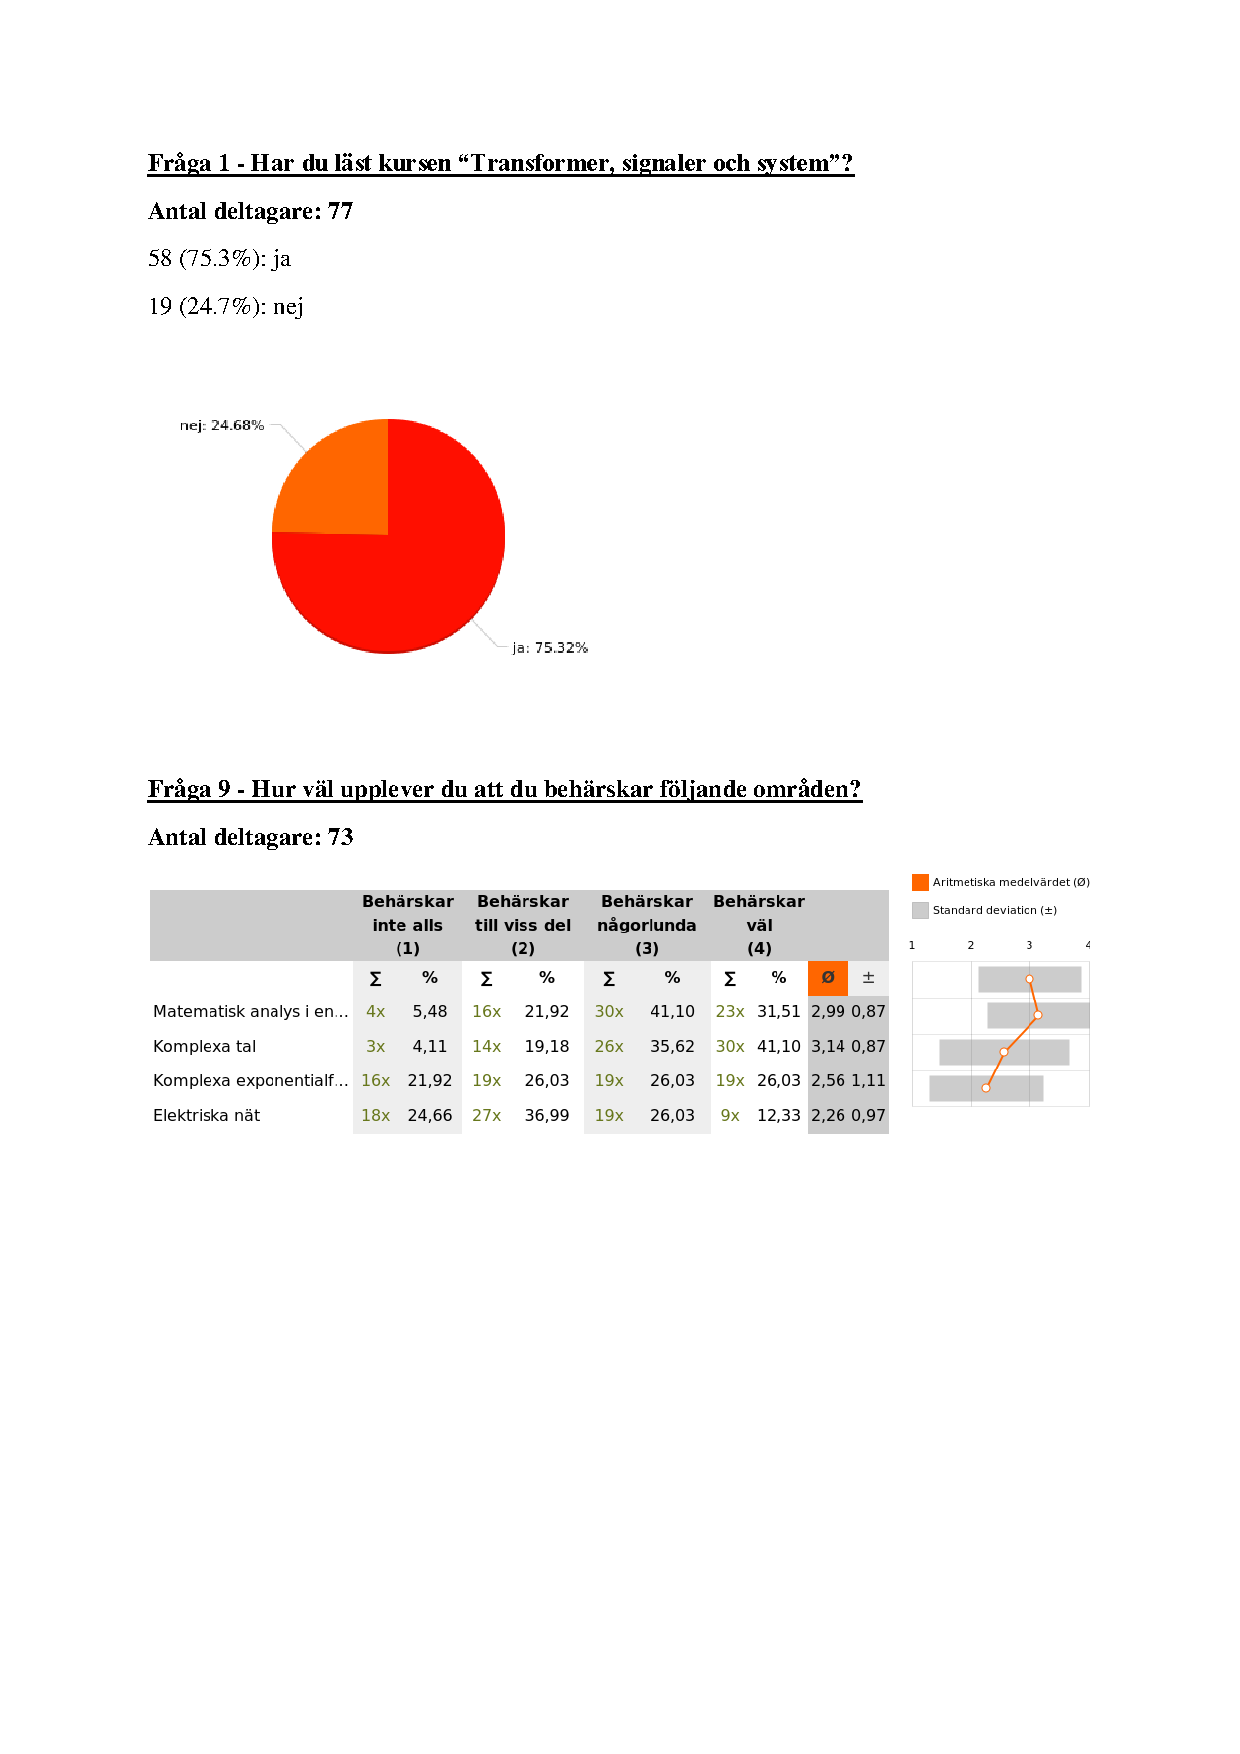
\includepdf[pages=-]{Bilagor/Bilaga1.pdf}
\newpage
%Todo: Det vore intressant att korrelera resultat med andra frågor.

\section{Bilaga 2}
\label{bil:exam_intervju}
Denna bilaga är en sammanfattning av den intervju projektgruppen höll
med Bo Egardt och Ants Silberberg. Bo och Ants har under flera år
varit både lärare och examinatorer i \gls{regler} respektive \gls{tss}
på Chalmers. Sammanfattningen är granskad och godkänd av både Bo och
Ants.

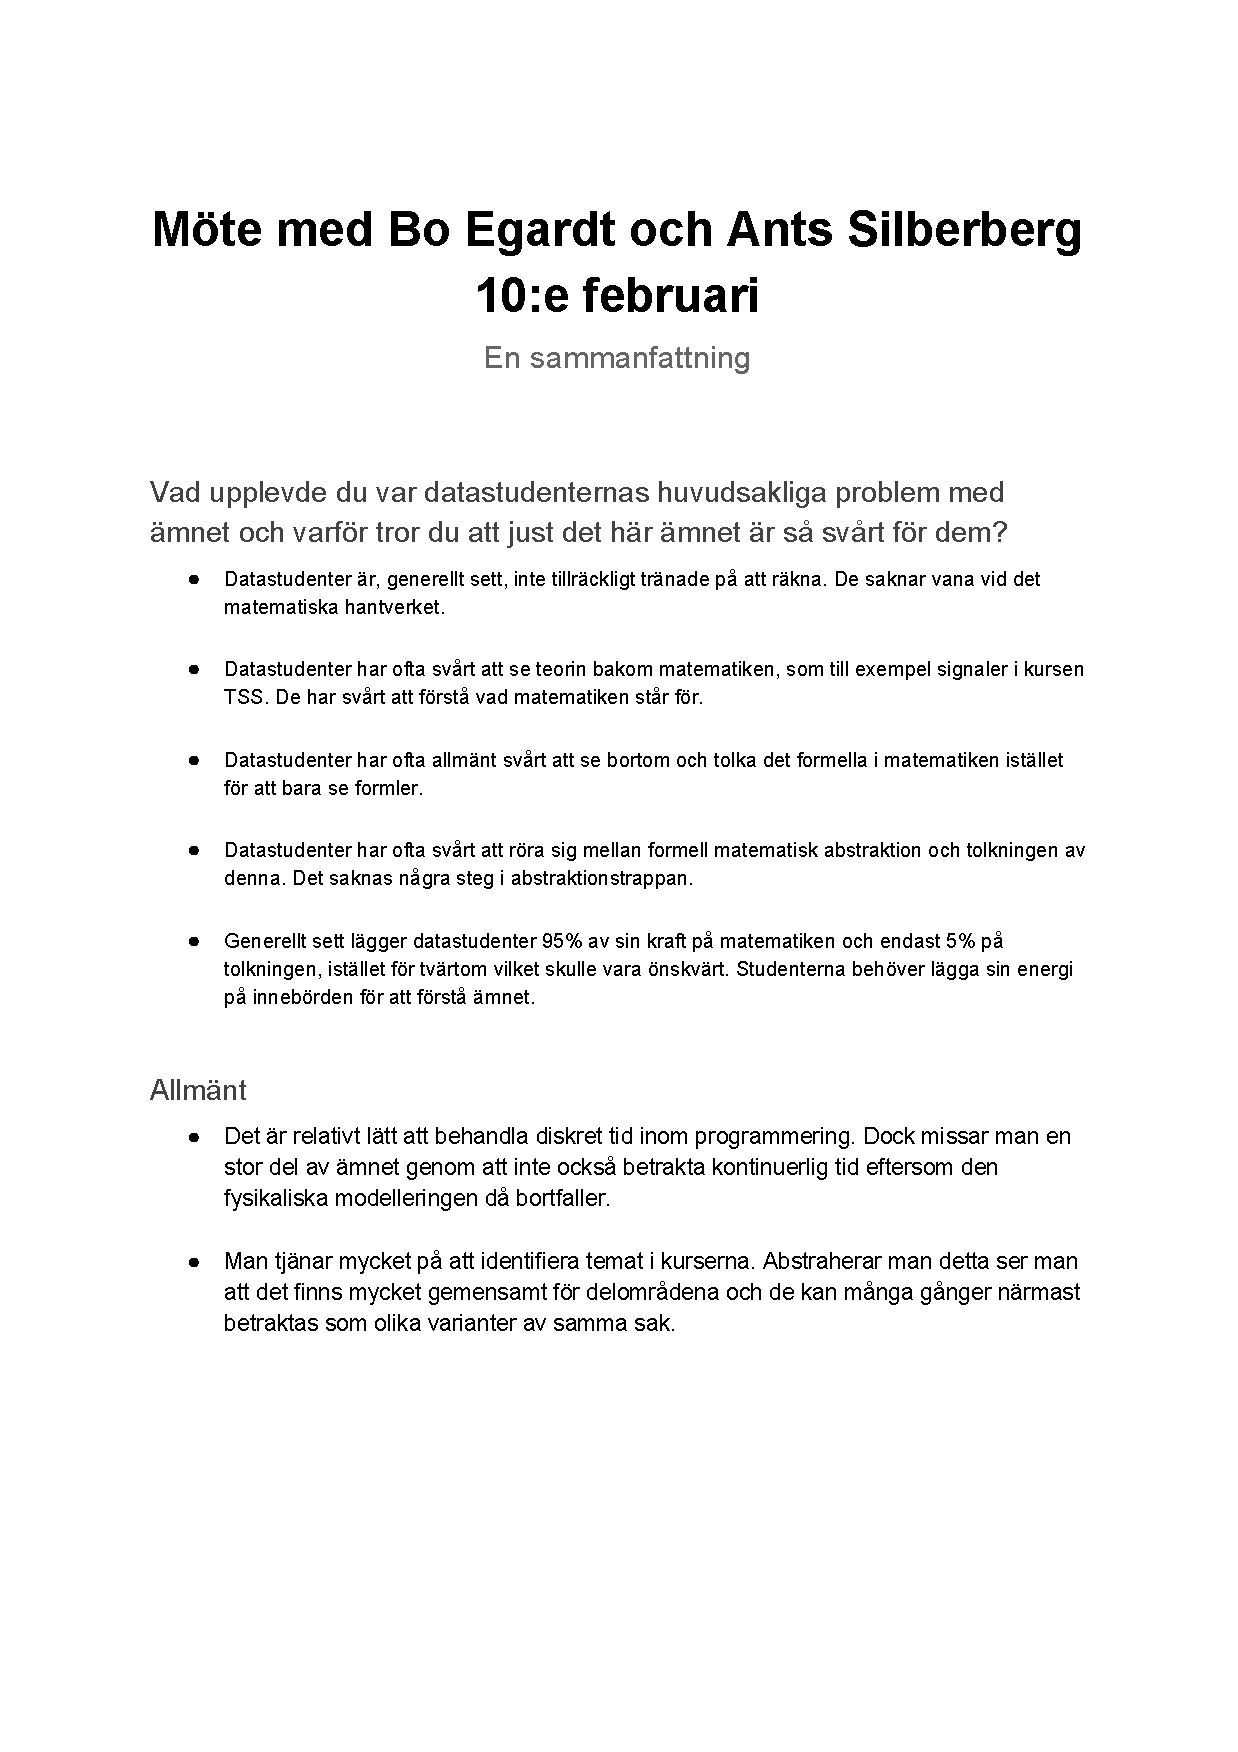
\includepdf[pages=-]{Bilagor/Bilaga2.pdf}
\newpage

\section{Bilaga 3}
\label{bil:3}
Denna bilaga är ett utdrag ur det läromaterial projektgruppen
utvecklat. Utdraget beskriver udda och jämna signaler och är hämtat
från avsnitt 2 i läromaterialet.

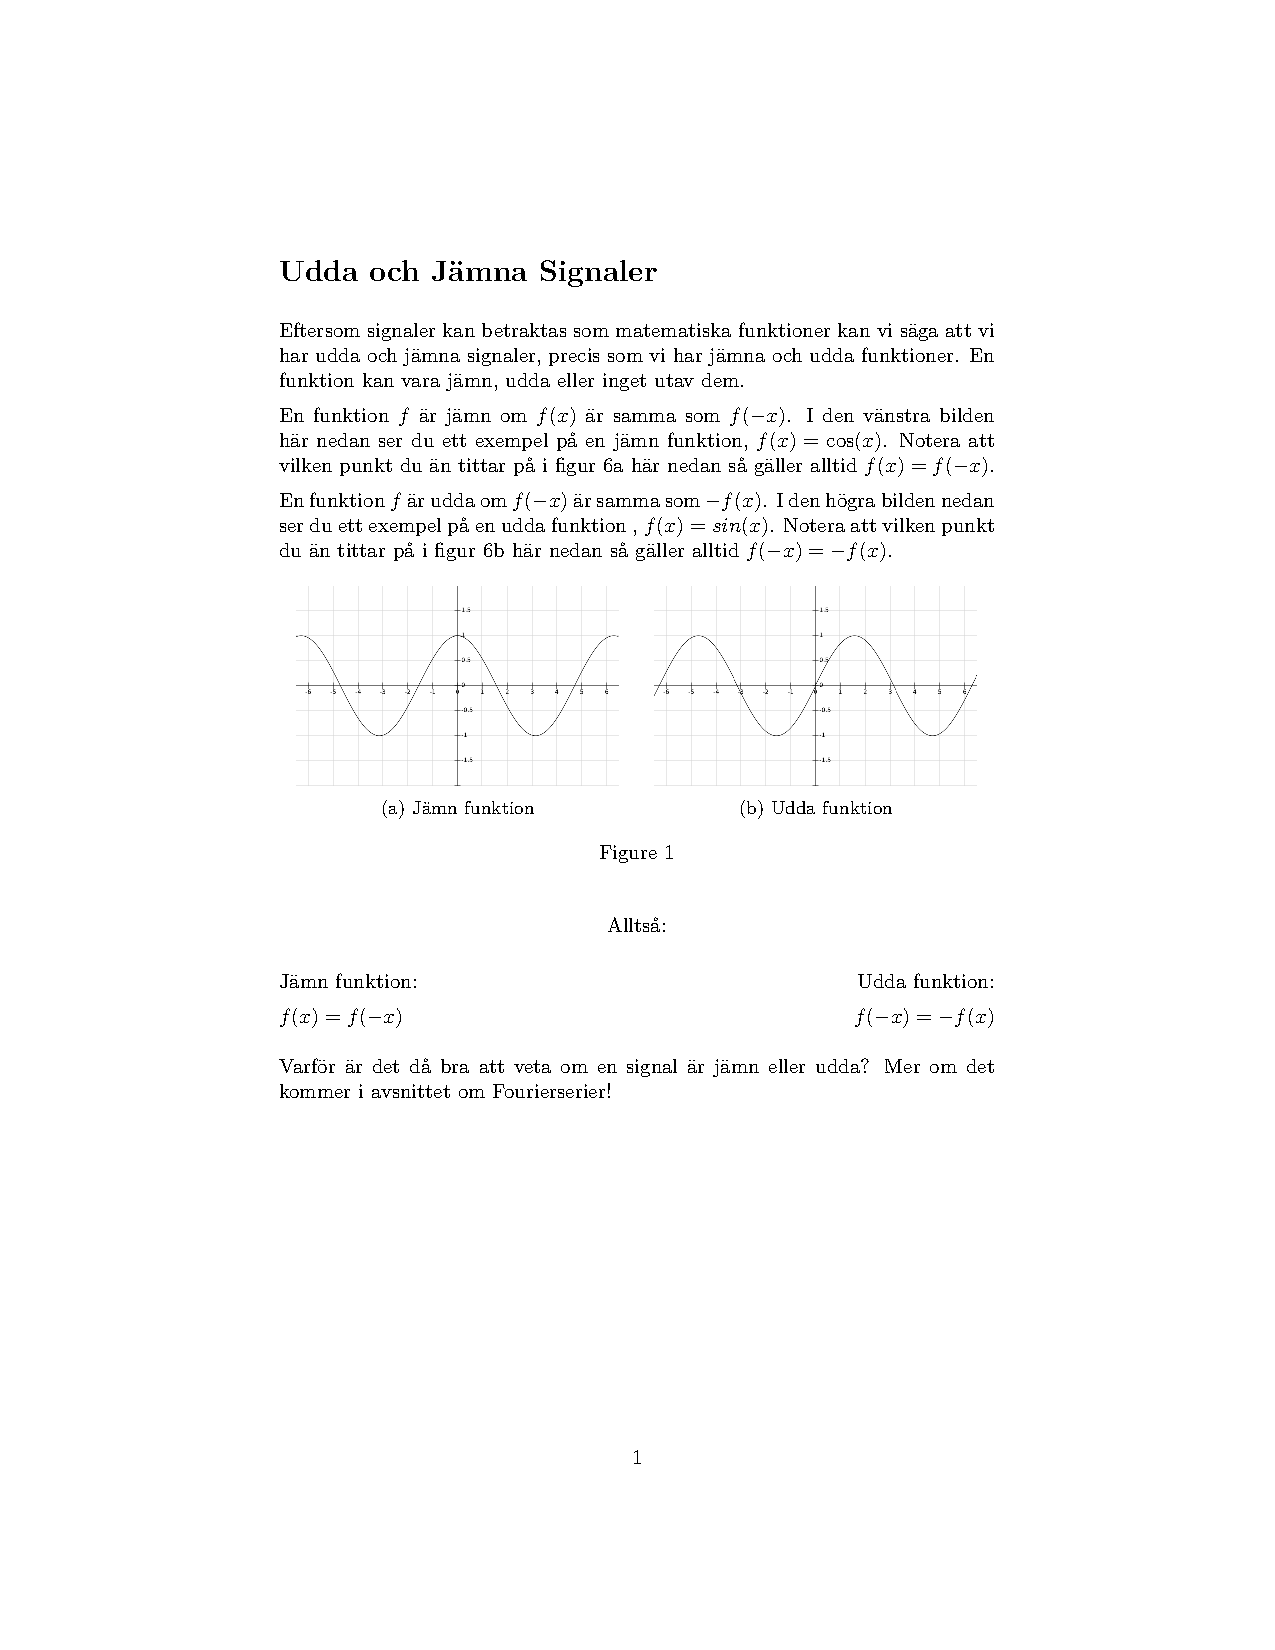
\includepdf[pages=-]{Bilagor/Bilaga3.pdf}
\end{document}
